\documentclass[../main.tex]{subfiles}




\begin{document}
























\chapter{Superfícies topològiques}

Aquest capítol estarà basat essencialment en els apunts que penja el professor cada setmana al Campus Virtual. Tot i així, com són bastant poc detallats, per dir-ho d'alguna manera, prendré també una font que m'ha sigut molt útils. Aquests són uns apunts del Jaume Aguadé \cite{aguade} que vaig trobar a partir de la pàgina web de l'Irene Llerena, anomenada ``Topología para usuarios'' \cite{topologiaparausuarios} (en castellà).

\section{Varietats topològiques}

Si comparem espais com puguin ser l'esfera, el tor o l'espai projectiu amb espais com el conjunt de Cantor, un espai groller o l'espai $\mathbb{Q}$, veiem que els primers tenen en comú que, a \textit{petita escala}, són indistingibles a l'espai euclidià $\mathbb{R}^n$. Els espais que tenen la propietat d'assemblar-se ``localment'' a l'espai euclidià tenen una enorme importància. Reben el nom de \textit{varietats}\footnote{En anglès, aquests objectes que estudiarem ara s'anomenen \textit{manifolds}. En aquest punt tenim un petit dèficit de lèxic respecte de l'anglès perquè les dues paraules angleses \textit{variety} i \textit{manifold} corresponen a una única paraula en català.} o, si volem evitar la confusió amb altres tipus de varietats, \textit{varietats topològiques}.

\subsection{El concepte de varietat topològica}

\begin{defi}
[Varietat topològica]\label{def:varietattopologica}\index{Varietat topològica} Una \textit{varietat topològica} de dimensió $n$ és un espai topològic $X$ que satisfà:
\begin{enumerate}[(i)]
    \item $X$ és de Hausdorff o $T_2$;
    \item $X$ admet una base numerable d'oberts;
    \item Cada punt de $X$ té algun entorn homeomorf a $\mathbb{R}^n$.
\end{enumerate}
\end{defi}

La darrera condició és equivalent a imposar que cada punt $p\in X$ tingui un entorn homeomorf a un subespai obert de $\mathbb{R}^n$, ja que si $p\in W$ i hi ha un homeomorfisme $f:W\rightarrow V$, amb $V\subseteq \mathbb{R}^n$ obert, llavors podem prendre un obert $U$ de $X$ amb $p\in U\subseteq W$ i una bola oberta $B$ de $\mathbb{R}^n$ tal que $f(p)\in B\subseteq f(U)$; aleshores $f^{-1}(B)$ és un entorn obert de $p$ homeomorf a $\mathbb{R}^n$.

Vegem-ne un exemple per aclarir el concepte. La Terra no és plana (s'assimila a l'esfera $S^2$ que no és homeomorfa al pla $\mathbb{R}^2$) però a cada punt de la terra podem dibuixar un ``mapa'' (que anomenarem \textit{carta local}\footnote{En francès, la paraula mapa es tradueix com \textit{carte}, i en italià \textit{carta}.}) que ens doni un homeomorfisme entre un entorn d'aquest punt de la Terra i un obert de $\mathbb{R}^2$. Després podem construir un \textit{atles}, que serà un conjunt de cartes locals que cobreixin tota a Terra\footnote{Un atles és un conjunt de mapes, com un llibre que conté tots els mapes.}. Aquests conceptes tenen sentit en una varietat qualsevol. Ara vegem-ne les definicions rigoroses.

\begin{defi}
[Carta local]\label{def:cartalocal}\index{Carta local} Si $M$ és una varietat topològica de dimensió $n$, una \textit{carta local} a $M$ és un parell $(U,\varphi)$ on $U$ és un obert de $M$ i $\varphi$ és un homeomorfisme de $U$ en un obert de $\mathbb{R}^n$. Llavors $\varphi$ es denota per $\varphi=(x_1,\ldots,x_n)$, on cada $x_i$ és una aplicació 
\begin{equation}
    \notag
    x_i:U\rightarrow\mathbb{R}
\end{equation}
Aquestes aplicacions s'anomenen \textit{coordenades locals}\index{Coordenades locals}.
\end{defi}

\begin{defi}
[Canvi de coordenades]\label{def:canvidecoordenades}\index{Canvi de coordenades} Si $(U_1,\varphi_1)$ i $(U_2,\varphi_2)$ són dues cartes locals i $U_1\cap U_2\not=\emptyset$, llavors l'homeomorfisme $\phi:(U_1,\varphi_1)\rightarrow (U_2,\varphi_2)$ definit com $\phi(x) = \varphi_2(\varphi_1^{-1}(x))$ s'anomena \textit{aplicació canvi de coordenades}.
\end{defi}

\begin{defi}
[Atles]\label{def:atles}\index{Atles} Una col·lecció
de cartes locals $\{(U_\lambda,\varphi_\lambda)\}_{\lambda\in \Lambda}$ tals que $\bigcup_{\lambda\in \Lambda} U_\lambda = M$ s'anomena \textit{atles}.
\end{defi}

\begin{defi}
[Varietat topològica amb vora]\label{def:varietattopologicaambvora}\index{Varietat topològica amb vora} Una \textit{varietat topològica de dimensió $n$ amb vora} és un espai de Hausdorff $M$ que admet una base d'oberts numerable i tal que cada punt de $M$ té algun entorn homeomorf a un subespai obert de $\mathbb{R}^n_+=\{(a_1,\ldots,a_n)\in\mathbb{R}^n\;:\;a_n\geq 0\}$. Anomenem \textit{interior}\label{def:interior}\index{Interior} de $M$ al subespai format pels punts $p\in M$ que tenen algun entorn homeomorf a $\mathbb{R}^n$ i \textit{vora}\label{def:vora}\index{Vora} de $M$ al subespai complementari. Llavors, l'interior de $M$ és una varietat de dimensió $n$ i la vora de $M$, que es denota per $\partial M$, és una varietat de dimensió $n-1$.
\end{defi}

\begin{defi}
[Varietat tancada]\label{def:varietattancada}\index{Varietat tancada} Una varietat (topològica) es diu \textit{tancada} si és compacta i sense vora. Adoptarem el conveni que ``varietat'', sense especificar, vol dir ``varietat sense vora''.
\end{defi}

\begin{ej}
[Exemples de varietats topològiques]\label{ej:varietatstopologiques} Vegem-ne alguns exemples.
\begin{enumerate}[(1)]
    \item Tot espai discret és una varietat de dimensió zero.
    \item $\mathbb{R}^n$ és una varietat de dimensió $n$. Ara bé, no som encara capaços de demostrar que $\mathbb{R}^n$ no sigui una varietat de dimensió $m$, per algun $m\not=n$.
    \item Un obert de $\mathbb{R}^n$ és una varietat de dimensió $n$. Més en general, un obert d'una varietat de dimensió $n$ és una varietat de dimensió $n$ també.
    \item L'esfera $S^n$ és una varietat compacta de dimensió $n$ i té un atles amb dues cartes locals. La projecció estereogràfica ens demostra que el complement d'un punt a $S^n$ és homeomorf a $\mathbb{R}^n$. Per tant, tot punt de $S^n$ té un entorn homeomorf a $\mathbb{R}^n$.
    \item Si $N$ és una varietat de dimensió $n$ i $M$ n'és una altra de dimensió $m$, llavors $N\times M$ és una varietat de dimensió $n+m$. En particular, el tor $S^1\times S^1$ és una varietat compacta de dimensió 2.
    \item L'espai projectiu $\mathbb{R}P^n$ és una varietat de dimensió $n$. La demostració és senzilla. Recordem que
    \begin{equation}
        \notag
        \mathbb{R}P^n = S^n\setminus\{-v\sim v\} .
    \end{equation}
    Donat $[x]\in\mathbb{R}P^n$, sigui $U:=B(x,\varepsilon)$ una bola de $S^n$ de radi prou petit perquè no hi hagi dos punts de $U$ que siguin diametralment oposats (o sigui antipodals). Recordem que la projecció $\pi:S^n\rightarrow \mathbb{R}P^n$ és oberta i tancada. Aleshores, la imatge de $U$ a $\mathbb{R}P^n$ és un obert homeomorf a $U$ i, per tant, a $\mathbb{R}^n$.
\end{enumerate}
\end{ej}


\subsection{Varietats amb vora}

Fem un petit incís en les varietats amb vora.

\begin{nota}
\label{nota:vora}\label{exercici3.1} Considerem $\mathbb{R}^n_+ = \{(x_1,\ldots,x_n)\in\mathbb{R}^n\;:\; x_n\geq 0\}$. Aquest espai no és homeomorf a $\mathbb{R}^n$, encara que ho pugui semblar.
\end{nota}
\begin{proof}
Anem a suposar que existeix un homeomorfisme $f:\mathbb{R}^n_+\rightarrow \mathbb{R}^n$ i arribem a una contradicció. Escollim el punt $O=(0,\ldots,0)\in\mathbb{R}^n_+$. Llavors $f$ es restringeix a un homeomorfisme $\mathbb{R}^n_+\setminus\{p\}\simeq \mathbb{R}^n_+\setminus\{f(p)\}$. Però $\mathbb{R}^n\setminus\{f(p)\}\simeq S^{n-1}$ i en canvi $\mathbb{R}^n_+\setminus\{p\}$ és contràctil.

Anem a demostrar que $\mathbb{R}^n_+\setminus\{p\}$ és contràctil. Observem que és homotòpicament equivalent a $\mathbb{R}^n_+\setminus B$ per retracció radial, on $B$ és una bola oberta de centre $p$. Aleshores, l'espai $\mathbb{R}^n_+\setminus B$ és homeomorf a $\mathbb{R}_+^n$ que és contràctil.
\end{proof}

\begin{prop}
\label{prop:voradernplus} Considerem el subespai $A = \{(x_1,\ldots,x_n)\in\mathbb{R}^n\;:\;x_n=0\}$. Aleshores $A = \partial\mathbb{R}^n_+$.
\end{prop}
\begin{proof}
Comprovem primer que $\partial\mathbb{R}^n_+\subseteq A$. Sigui $p\in\partial\mathbb{R}^n_+$ i posem $p = (p_1,\ldots,p_n)$. Si $p_n>0$, llavors existeix una petita bola oberta centrada al punt $p$ i continguda a l'interior de $\mathbb{R}^n_+$. Això ens diu que $p$ té un entorn homeomorf a $\mathbb{R}^n$, contràriament a la hipòtesi que $p\in\partial\mathbb{R}^n_+$. Per tant, $p_n=0$ i això implica que $p\in A$.

Anem a demostrar la inclusió contrària. Si $q\in A$ té algun entorn obert $U$ homeomorf a $\mathbb{R}^n$, llavors repetim el mateix raonament de l'anterior observació (\ref{nota:vora}). Considerem un homeomorfisme $f:U\rightarrow \mathbb{R}^n$, que es restringeix a un homeomorfisme $U\setminus\{q\}\simeq \mathbb{R}^n\setminus\{f(q)\}$, i observem que $U\setminus\{q\}\simeq U\setminus B\simeq U$ (equivalència homotòpica), on $B$ és una petita bola centrada a $q$ i continguda a $U$. Amb aquesta contradicció hem demostrat que $A\subseteq \partial\mathbb{R}^n_+$, tal com volíem.
\end{proof}

Sigui $M$ una varietat amb vora tal que $\dim M = n$. Suposem que $n\geq 1$. Llavors l'interior de $M$ està format pels punts de $M$ que tenen algun entorn homeomorf a $\mathbb{R}^n$ i, per tant, l'interior de $M$ és una varietat topològica de dimensió $n$ per definició.

Ara bé, què és la vora de $M$, $\partial M$? Anem a veure que és una varietat de dimensió $n-1$.

\begin{prop}
\label{prop:voraesvarietat} Sigui $M$ una varietat de dimensió $n\geq 1$. Aleshores $\partial M$ és una varietat de dimensió $n-1$.
\end{prop}
\begin{proof}
Prenem un punt $p\in\partial M$. Escollim un entorn obert $U$ de $p$ a $M$ amb un homeomorfisme $f:U\rightarrow V$ on $V$ és un obert de $\mathbb{R}^n_+$. Llavors $f(p)\in \partial \mathbb{R}^n_+$, ja que en cas contrari hi hauria una bola oberta $B$ a $\mathbb{R}^n$ tal que $f(p)\in B\subseteq V$ i llavors les relacions $p\in f^{-1}(B)\subseteq U$ contradirien el fet que $p\in\partial M$. Aleshores, $f(p)\in V\cap \partial\mathbb{R}_+^n$. Observem que $V\cap \partial\mathbb{R}^n_+$ es correspon amb un obert de $\mathbb{R}^{n-1}$ a través de l'homeomorfisme natural $\partial \mathbb{R}^n_+\simeq \mathbb{R}^{n-1}$. Llavors, $f^{-1}(V\cap\partial \mathbb{R}^n_+)$ és un entorn obert de $p$ a $\partial M$ que és homeomorf a un obert de $\mathbb{R}^{n-1}$.
\end{proof}

Finalment, recordem que si $\mathbb{R}^n\simeq \mathbb{R}^m$, on $\simeq$ indica aquí un homeomorfisme, aleshores teníem que $n=m$. Veurem ara que dues varietats topològiques amb vora que siguin homeomorfes (és a dir, tals que existeixi un homeomorfisme d'una a l'altra) tindran la mateixa dimensió.

\begin{prop}
\label{prop:varietatsambvorahomeomorfes} Sigui $f:M\rightarrow N$ un homeomorfisme entre varietats amb vora $M$ i $N$. Llavors $\dim M=\dim N$.
\end{prop}
\begin{proof}
Considerem l'homeomorfisme $f:M\rightarrow N$ que, en particular, és un homeomorfisme local. Sigui $p\in \partial M$. Si $f(p)$ tingués un entorn obert $W$ homeomorf a $\mathbb{R}^n$, llavors $f^{-1}(W)$ seria un entorn obert de $p$ homeomorf a $\mathbb{R}^n$. Per tant, $f(p)\in\partial N$. Per simetria, tot punt de $\partial N$ és a la imatge d'algun punt de $\partial M$. Per tant, $f$ es restringeix a un homeomorfisme $\partial M\simeq \partial N$ i aleshores els seus complementaris també són homeomorfs, és a dir, l'interior de $M$ és homeomorf a l'interior de $N$.
\end{proof}






\subsection{Varietats connexes}

Evidentment, una varietat pot ser connexa o no ser-ho. Si $M$ i $N$ són varietats, és clar que la unió no-connexa $M\sqcup N$ és també una varietat i no és connexa. El teorema següent ens diu que si coneixem les varietats connexes, ja coneixem totes les varietats\footnote{Per entendre millor el teorema que ve a continuació, recordem que tot espai és la unió disjunta dels seus components connexos, però no tot espai és unió no-connexa dels seus components connexos. Per exemple, els components connexos de $\mathbb{Q}$ són els punts, però una unió no-connexa de punts és un espai discret i $\mathbb{Q}$ no ho és. Aquest fenomen també es pot donar en espais compactes: els components connexos del conjunt de cantor $\mathcal{C}$ (que és compacte) són els punts, però $\mathcal{C}$ no és discret. El que diu el teorema és que aquesta situació no es pot donar a les varietats topològiques.}.

\begin{ter}
\label{ter:varietatsconnexes} Sigui $M$ una varietat de dimensió $n$ i siguin $M_i$, $i\in I$, els seus components connexos.
\begin{enumerate}[(1)]
    \item Els $M_i$ són oberts de $M$.
    \item $I$ és numerable. Si $M$ és compacta, $I$ és finit.
    \item Cada $M_i$ és una varietat de dimensió $n$.
    \item $M$ és la unió no-connexa dels seus components connexos: $M= \bigsqcup_{i\in I} M_i$.
\end{enumerate}
\end{ter}
\begin{proof}
Cada punt de $M$ té un entorn homeomorf a $\mathbb{R}^n$. Per tant, cada punt de $M$ té un entorn connex. Això implica immediatament que cada $M_i$ és obert. Com que un obert d'una varietat és una varietat, tenim que cada $M_i$ és una varietat. La quarta condició és certa per a tot espai en què els components connexos siguin oberts. Si $I$ no fos numerable, $M$ no podria tenir una base numerable d'oberts. Si $I$ és infinit, és evident que $M$ no pot ser compacta.
\end{proof}

En conclusió, tota varietat és unió no-connexa numerable de varietats connexes. A partir d'ara, doncs, només ens preocuparem per les varietats connexes.


\subsection{Varietats de dimensió 1}

Essencialment, només hi ha dues varietats connexes de dimensió 1: la recta i la circumferència. Aquestes són diferents ja que una és compacta i l'altra no. Veurem, doncs, que qualsevol varietat de dimensió 1 serà homeomorfa a una d'aquestes dues.

\begin{ter}
\label{ter:varietatsdedim1} Si $M$ és una varietat connexa de dimensió 1, aleshores $M\simeq \mathbb{R}$ o bé $M\simeq S^1$, on $\simeq$ indica homeomorfisme.
\end{ter}
\begin{proof}
La farem en diverses etapes.
\begin{itemize}
    \item Evidentment, si $M$ es pot recobrir amb una única carta local, aleshores, $M\simeq \mathbb{R}$ i hem acabat.
    \item El pas clau de la demostració és entendre què passa si $M$ es pot recobrir amb dues cartes locals.
    
    Suposem que $M = U\cup V$, on $U,V\varsubsetneq M$ són oberts de $M$, cadascun d'ells homeomorf a $\mathbb{R}$ a través dels homeomorfismes següents:
    \begin{equation}
        \notag
        \phi:U\overset{\simeq}{\longrightarrow}\mathbb{R},\qquad \psi:V\overset{\simeq}{\longrightarrow} \mathbb{R}.
    \end{equation}
    Com que $M$ és connexa, aquests dos oberts no poden ser disjunts. Considerem
    \begin{equation}
        \notag
        A:=\phi(U\cap V)\subset\mathbb{R}
    \end{equation}
    que és un obert de $\mathbb{R}$ i, per tant, una varietat de dimensió 1. Pel teorema (\ref{ter:varietatsconnexes}), els seus components connexos són oberts connexos de $\mathbb{R}$, és a dir, intervals oberts. El pas següent consisteix en veure que aquests intervals no poden ser acotats.
    
    Suposem que, per exemple, $A$ tingués un component connex de la forma $(a,b)$, amb $a,b\in\mathbb{R}$. Considerem
    \begin{equation}
        \notag
        \phi^{-1}(a,b)\subset U\cap V\subset V
    \end{equation}
    i $\phi^{-1}([a,b])$ és tancat de $M$ perquè és compacte. Com que $\phi^{-1}(a,b)$ és un obert i tancat de $V\simeq \mathbb{R}$, tenim que $\phi^{-1}(a,b)=V$ i això implica que $V\subset U$ i $U=M$, contradicció.
    
    Hem vist que els components connexos de $A$ són intervals no acotats (diferents de tota la recta $\mathbb{R}$). Com que els components connexos han de ser disjunts, això només és possible en dos casos:
    \begin{enumerate}[i.]
        \item $A$ és connex de la forma $(-\infty,a)$ o bé $(a,+\infty)$, per algun $a\in \mathbb{R}$, o bé
        \item $A$ és de la forma $(-\infty,a)\cup (b,+\infty)$, per uns certs $a,b\in\mathbb{R}$ tals que $a<b$.
    \end{enumerate}
    Com que $B:=\psi(U\cap V)\simeq \phi(U\cap V) = A$, el mateix podem dir de $B$.
    
    Ara, és relativament senzill en el primer cas construir un homeomorfisme $M\simeq \mathbb{R}$ i en el segon cas construir un homeomorfisme $M\simeq S^1$. Deixem aquests detalls com exercici.
    
    \item Suposem ara que $M$ es pot recobrir amb un nombre finit de cartes locals $U_1,\ldots,U_n$. Demostrem el teorema per inducció sobre $n$. Si $n=1$ és trivial. Si $n=2$ és el que hem fet fins ara. Apliquem el teorema a $M':=U_1\cup \cdots\cup U_{n-1}$. Si $M'\simeq \mathbb{R}$, tenim que $M'$ és una carta local de $M$ i $M$ es pot recobrir per dues cartes locals. Si $M'\simeq S^1$, aleshores $M'$ és compacte, per tant, és tancat a $M$  com que també és obert, tindrem $M = M'\simeq S^1$ i hem acabat.
    
    \item Ens quedaria el cas general en què $M$ no es pot recobrir amb un nombre finit de cartes locals. En primer lloc, és fàcil adonar-se que el segon axioma de numerabilitat implica que $M$ es pot recobrir amb una quantitat numerable de cartes locals, és a dir,
    \begin{equation}
        \notag
        M = U_1\cup U_2\cup U_3\cup \cdots
    \end{equation}
    Pel raonament del punt anterior, $\forall n>1$ tenim
    \begin{equation}
        \notag
        V_n:=U_1\cup\cdots\cup U_n\simeq \mathbb{R}\simeq (0,1)
    \end{equation}
    i és senzill ``enganxar'' tots aquests homeomorfismes per obtenir un homeomorfisme $M\simeq\mathbb{R}$.
\end{itemize}
\end{proof}









\section{Superfícies topològiques}

Aquest capítol rep el títol de ``Superfícies topològiques'' però fins ara no n'hem parlat. En realitat, és perquè una superfície topològica no és més que una varietat topològica de dimensió 2. És per això, que he cregut convenient fer primer una secció que expliqués el concepte de varietat topològica en general, per després reduir a dimensió 2 i centrar-nos en les superfícies topològiques.

\begin{defi}
[Superfície topològica]\label{def:superficietopologica}\index{Superfície topològica} Una \textit{superfície topològica} és una varietat topològica de dimensió 2. És a dir, és un espai topològic que verifica el segon axioma de numerabilitat, que és de Hausdorff i que localment és homeomorf a $\mathbb{R}^2$.
\end{defi}

De vegades, per simplificació i per abús del llenguatge, direm només ``superfície'' per referir-nos a ``superfície topològica'', sempre i quan no doni pas a una confusió amb superfícies d'altra naturalesa.

\begin{ej}
El pla $\mathbb{R}^2$ n'és l'exemple més elemental de superfície topològica. Vegem-ne d'altres.
\begin{enumerate}[(1)]
    \item Les quàdriques no degenerades de $\mathbb{R}^3$ com els el·lipsoides, els cilindres, els hiperboloides, etc. en són altres exemples clàssics.
    \item Entre les superfícies compactes, l'esfera i el tor són les més elementals. Ambdues superfícies es poden obtenir a partir d'un polígon del pla (concretament $[0,1]\times[0,1]$ si fem algunes transformacions) per identificació d'arestes. 
    
    En efecte, si considerem un quadrat de vèrtexs $ABCD$, l'esfera s'obté identificant el costat $AD$ amb el costat $AB$ i els costat $BC$ amb el costat $DC$. D'altra banda, el tor s'obté identificant el costat $AD$ amb $BC$, i el costat $AB$ amb $DC$. Un dibuix il·lustratiu és el següent\footnote{És interessant veure-ho en 3 dimensions en un vídeo que ho il·lustri, al youtube.}:
    \begin{equation}
        \notag
        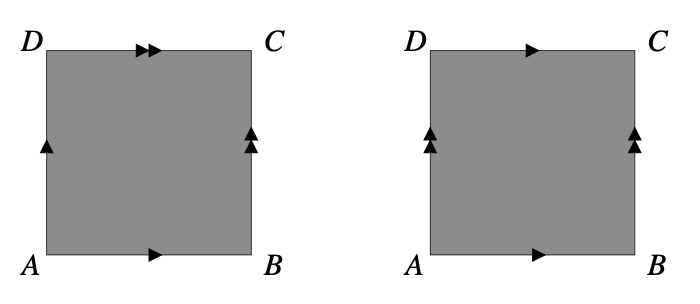
\includegraphics[scale = 0.5]{fotos_topo_2/esferaitor.png}
    \end{equation}
\end{enumerate}
\end{ej}

Ja vam veure en diversos exemples anteriors que es podien obtenir determinades superfícies fent el quocient d'un quadrat (per exemple $I^2 = [0,1]\times[0,1]$) per unes certes identificacions entre els punts dels costats. El tor, l'esfera, el pla projectiu i l'ampolla de Klein són exemples ben coneguts que es poden obtenir d'aquesta manera (com es va veure a l'assignatura Topologia). Podem fer coses similars amb un polígon (``ple''), és a dir, estendre aquesta idea d'un quadrat a un polígon més general. Podem prendre un polígon $P\subset \mathbb{R}^2$ i fer el quocient per algunes identificacions entre els seus costats. Normalment, aquestes identificacions es representen gràficament orientant els costats i anomenant amb una mateixa lletr els costats que identifiquem, com a la figura següent
\begin{figure}
    \centering
    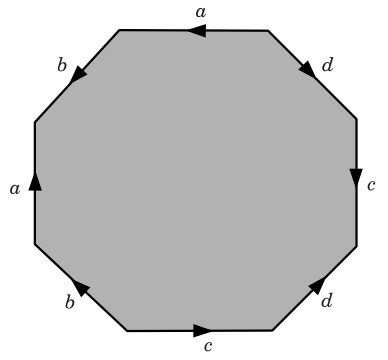
\includegraphics[scale = 0.6]{fotos_topo_2/octogonid.png}
    \caption{Un octògon amb els costats identificats. Captura de pantalla de \cite{aguade}}
    \label{fig:octogon}
\end{figure}
que representa un octògon amb els costats identificats.

En cada cas, l'espai quocient està perfectament ben definit, però pot ser que no sigui una superfície. En una superfície, cada punt ha de tenir un entorn homeomorf a un disc $D^2$ (que seria un obert de $\mathbb{R}^2$). Per als punts de l'interior del polígon $P$, això és clar, però per als punts dels costats (de la vora) de $P$, dependrà de com siguin les identificacions i, en cada cas, cal comprovar amb paciència si els punts interiors de les arestes tenen entorns homeomorfs a $D^2$ i si això també és cert per als vèrtexs. Per exemple, si volem que el quocient sigui una superfície, és clar que una condició necessària és que els costats estiguin identificats dos a dos, és a dir, que cada costat del polígon $P$ estigui identificat amb un únic costat de $P$. En particular, això és equivalent a que el nombre de costats de $P$ sigui parell\footnote{Sembla evident que si hi ha tres arestes, per exemple, identificades, el quocient no pot ser una superfície. Tot i així la demostració no és del tot trivial i utilitza el teorema de la corba de Jordan.}. També és cert, encara que no és evident, que aquesta condició és suficient. Tot això ho veurem de forma més rigorosa.

Per exemple, en el cas de l'octògon $P$ de la figura (\ref{fig:octogon}), es pot comprovar que el quocient és una superfície que es pot representar com un subespai de $\mathbb{R}^3$ (figura \ref{fig:transformacionoctogon})
\begin{figure}
    \centering
    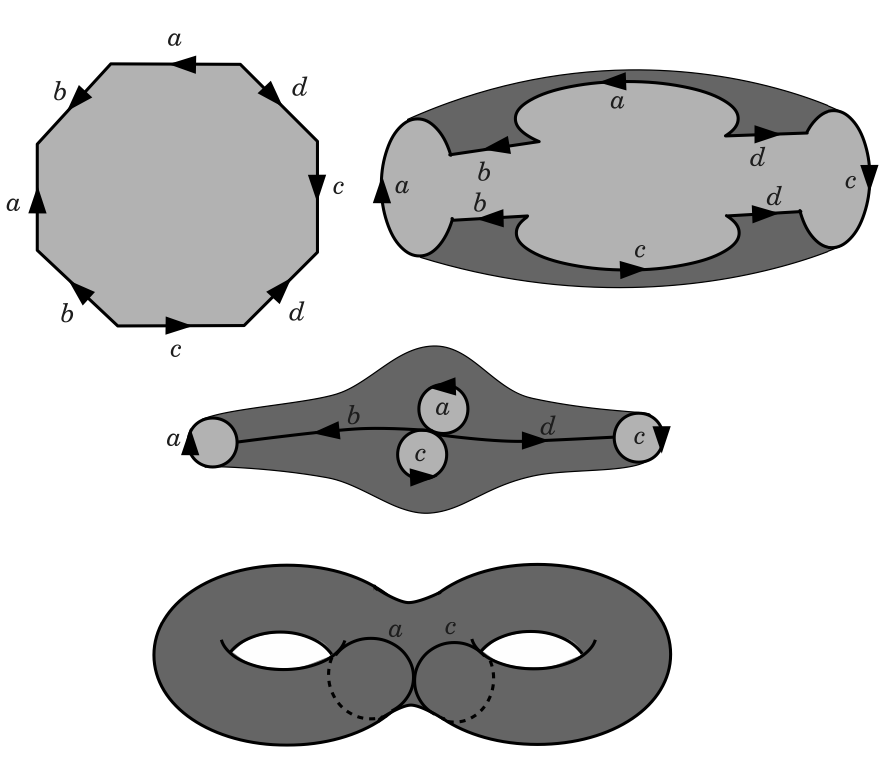
\includegraphics[scale = 0.5]{fotos_topo_2/transformacionoctogon.png}
    \caption{El doble tor a partir d'un octògon amb els costats identificats (Captura de pantalla de \cite{aguade})}
    \label{fig:transformacionoctogon}
\end{figure}
que s'anomena el ``doble tor''. Però hi pot haver exemples en que s'obtinguin superfícies que, com el pla projectiu o l'ampolla de Klein, no siguin subespais de $\mathbb{R}^3$.

Aquestes construccions es poden generalitzar a una dimensió més. Per exemple, si agafem un políedre (``ple'') de $\mathbb{R}^3$ i identifiquem les cares d'alguna manera, l'espai quocient podria resultar que és una varietat de dimensió 3. Un exemple fàcil consisteix en prendre un cub $I^3 = [0,1]^3$ i identificar els seus costats de manera que l'espai quocient sigui un tor de dimensió 3 $T^3 = S^1\times S^1\times S^1$. Un exemple més sofisticat i molt més interessant és el de l'esfera de Poincaré\footnote{Aquesta varietat de dimensió 3 la va descobrir Henri Poincaré el 1904 com a contraexemple a la primera versió de la famosa \textit{conjectura de Poincaré}. A la vista d'aquest contraexemple, el mateix Poincaré va modificar la seva conjectura i la nova versió va ser un dels problemes fonamentals de les matemàtiques fins l'any 2002 en què Grigori Perelman va demostrar que la conjectura és correcta. Si llegim l'obra original de Poincaré, observem que no va mai presentar el seu problema com una conjectura, sinó com una pregunta. \begin{quote}
    «Est-il possible que le groupe fondamentale de $V$ se réduise à la substitution identique, et que pourtant $V$ ne soit pas simplement connexe? [\ldots] Mais cette question nous entrainerait trop loin.»
\end{quote} I tant! Han calgut 100 anys d'avenços de la topologia i la geometria per respondre aquesta pregunta. Font \cite{aguade}}. Això, però, quedarà per a una altra assignatura, ja que, per ara, ens centrarem en les superfícies poligonals.


\subsection{Superfícies poligonals}

En aquest apartat farem el que hem descrit anteriorment: estudiarem la construcció de superfícies a partir de la identificació dels costats orientats d'un polígon arbitrari.

Considerem un polígon regular del pla, $P$, amb un nombre parell de costats $2n$. Numerarem els vèrtex de forma creixent, és a dir, $p_1,\ldots,p_{2n}$ segons el sentit antihorari, i agruparem les arestes orientades per parells, és a dir, $[p_i,p_{i+1}]$ representa l'aresta de vèrtexs $p_i$ i $p_{i+1}$.

\begin{defi}
[Afinitat bijectiva d'arestes]\label{def:afinitatbijectiva}\index{Afinitat bijectiva d'arestes} Utilitzant la notació descrita dels polígons i les seves arestes, denotarem
\begin{equation}
    \notag
    \tau_{ij}:[p_i,p_{i+1}]\longrightarrow [p_j,p_{j+1}]
\end{equation}
una \textit{afinitat bijectiva}, que voldrà dir que les arestes $[p_i,p_{i+1}]$ i $[p_j,p_{j+1}]$ estan \textit{aparellades}\index{Arestes aparellades}. Observem que només hi ha dues afinitats possibles:
\begin{enumerate}[(I)]
    \item Si $\tau_{ij}(p_i)=p_j$ i, necessàriament, $\tau_{ij}(p_{i+1})=p_{j+1}$, direm que $\tau_{ij}$ \textit{conserva l'orientació}
    \item Si $\tau_{ij}(p_i) = p_{j+1}$ i, necessàriament, $\tau_{ij}(p_{i+1}) = p_j$, direm que $\tau_{ij}$ \textit{inverteix l'orientació}.
\end{enumerate}
\end{defi}


A continuació veurem el que ja hem comentat abans, que si tenim un nombre parell de costats a un polígon $P$ i hi identifiquem aquests costats dos a dos, d'una manera determinada, podem aconseguir una superfície topològica. Amb les identificacions $\tau_{ij}$ descrites això pot ser possible i ho provarem al següent teorema.

\begin{ter}
\label{ter:superficiecompactaiconnexa} Considerem l'espai topològic $X$ que s'obté quan identifiquem les arestes dos a dos segons les afinitats (\ref{def:afinitatbijectiva}), és a dir, que $X$ és l'espai quocient de $P$ per la relació d'equivalència $R$ generada per la relació
\begin{equation}
    \notag
    x\simeq \tau_{ij}(x),\quad \forall x\in \partial P
\end{equation}
Llavors $X$ és una superfície topològica, compacta i connexa.
\end{ter}
\begin{proof}
La compacitat i la connexió es dedueixen de les mateixes propietats de $P$, ja que $\pi:P\rightarrow X$ (la projecció) és una aplicació d'identificació. Així mateix $X$ verifica el segon axioma de numerabilitat. El que cal provar és que $X$ és localment homeomorf a $\mathbb{R}^2$ i és de Hausdorff.

Observem que podem distingir tres tipus de punts de $X$: els de $\pi(P)$, que només tenen una antiimatge per $\pi$; els de $\pi(\partial P\setminus\{p_1,\ldots,p_{2n}\})$, que tenen dues antiimatges a $P$; i els que corresponen als vèrtexs $p_i$, amb un nombre indeterminat d'antiimatges entre 1 i $2n$. En qualsevol cas, la antiimatge d'un punt de $X$ per $\pi$ és un nombre finit de punts.

Per veure que $X$ és localment $\mathbb{R}^2$ hem de fer un estudi per a cadascun dels tipus de punts.
\begin{enumerate}
    \item Si $x = \pi(p)$ és imatge d'un punt interior de $P$ aleshores el resultat és immediat ja que en un entorn prou petit de $p$ l'aplicació $\pi$ és homeomorfisme.
    
    \item Si $x\in X$ és imatge d'un punt d'una aresta que no és un vèrtex, $x$ tindrà dues antiimatges, $q_1$ i $q_2$, ambdues sobre dos costats de $P$ identificats per $\pi$. Si prenem ara discs $D_1,D_2$ del pla centrats en $q_1,q_2$ i de radi prou petit $\varepsilon$ per tal que no continguin cap vèrtex de $P$, aleshores $D = \pi[(D_1\cap P)\cup (D_2\cap P)]$ és homeomorf a un disc de $\mathbb{R}^2$ (veure imatge \ref{fig:d1d2})
    \begin{figure}
        \centering
        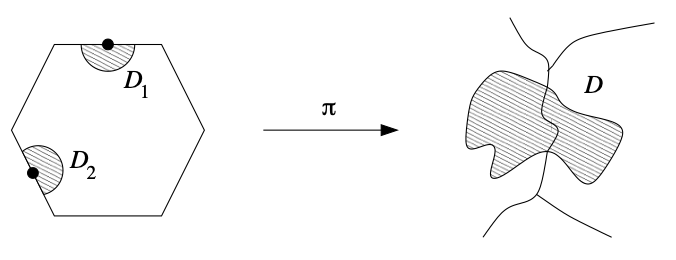
\includegraphics{fotos_topo_2/d1d2.png}
        \caption{Disc al voltant d'un punt en la imatge de dues arestes.}
        \label{fig:d1d2}
    \end{figure}
    \item Sigui ara $x$ un punt de $X$ que és la imatge de $r$ vèrtexs de $P$, $p_{i_1},\ldots,p_{i_r}$. Com e el cas anterior prenem discs $D_{i_j}$ de $\mathbb{R}^2$ centrats en els punts $p_{i_j}$, $1\leq j\leq r$, de radi fixat $\varepsilon$ prou petit per tal que no continguin altres vèrtexs de $P$ que $p_{i_1},\ldots,p_{i_r}$, i notem de la mateixa manera les corresponents interseccions amb $P$, $1\leq j\leq r$. Com els costats de $P$ estan identificats a parells, podem suposar ordenats els punts $p_{i_j}$ de forma que cada $D_{i_j}$ tingui un costat en comú amb el disc anterior i l'altre amb el posterior. És un exercici comprovar aleshores que $D = \pi\left(\bigcup_{1\leq j\leq r}D_{i_j}\right)$ és un entorn de $x$ homeomorf a un disc del pla (veure \ref{fig:discos})
    \begin{figure}
        \centering
        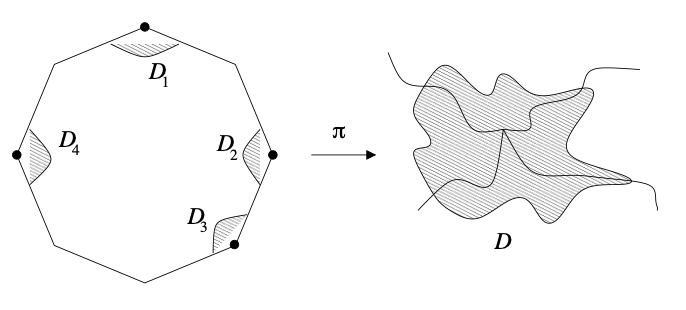
\includegraphics{fotos_topo_2/discos.png}
        \caption{Disc al voltant d'un punt imatge de $r$-vèrtexs}
        \label{fig:discos}
    \end{figure}
    
    Observi's que aquest darrer raonament no és vàlid quan un vèrtex no s'identifica a cap altre. En aquest cas, si $D$ és la intersecció de $P$ amb un disc que no conté cap altre vèrtex, les arestes de $D$ s'identifiquen per donar l'entorn de $x$ corresponent.
\end{enumerate}

Utilitzant oberts com els descrits en la prova anterior que $X$ és localment homeomorf a $\mathbb{R}^2$, prou petits, es demostra que $X$ és un espai de Hausdorff.
\end{proof}

\begin{defi}
[Superfície poligonal]\label{def:superficiepoligonal}\index{Superfície poligonal} Sigui $X$ una superfície compacta. Direm que $X$ és una \textit{superfície poligonal} si existeix un polígon regular $P$ amb un nombre parell de costats, i un aparellament dels costats orientats, tal que $X$ és homeomorfa a la superfície quocient $P/\sim$.
\end{defi}

És clar que les superfícies poligonals que s'obtenen depenen de com s'hagin aparellat els costats del polígon $P$. Precisarem aquesta dependència de la forma següent: sigui $P$ un polígon regular de $2n$ costats, i suposem que els costats estan agrupats per parells. A cada costat li assignarem una lletra $a,b,c,\ldots$, i al costat associat li assignarem la mateixa lletra si s'identifiquen per l'afinitat que conserva l'orientació, o la mateixa lletra amb l'exponent -1 si s'identifiquen per l'afinitat que inverteix l'orientació. Aleshores, l'aparellament de les arestes de $P$ queda determinat per la \textit{paraula} que correspon a la juxtaposició de les lletres de les arestes, començant per una aresta i seguint en ordre antihorari.

\begin{defi}
[Paraula]\label{def:paraula} En el context anterior, diem que $A$ és una paraula de longitud $n$, $A(a_1,\ldots,a_n)$, si conté $n$ lletres, $a_1,\ldots,a_n$, cadascuna de les quals apareix dues vegades en la forma
\begin{equation}
    \notag
    \ldots a_i\ldots a_i\ldots \quad \text{o}\quad \ldots a_i\ldots a_i^{-1}\ldots 
\end{equation}
Denotarem per $X_A$ la superfície que li correspon segons la construcció anterior.
\end{defi}

\begin{ej}
Vegem-ne exemples de paraules i de les seves superfícies topològiques associades.
\begin{enumerate}[(1)]
    \item El tor $\mathbb{T}^2$ correspon a la paraula $aba^{-1}b^{-1}$.
    \item L'ampolla de Klein correspon a la paraula $abab^{-1}$.
    \item L'esfera $S^2$ correspondrà a la paraula $abb^{-1}a^{-1}$.
    \item El pla projectiu real a la paraula $abab$.
\end{enumerate}
\end{ej}

\begin{nota}
A vegades, per simplificar les paraules, s'agrupen lletres. Per exemple, l'esfera hem vist que era $abb^{-1}a^{-1}$. Llavors, podríem fer $c:=ab$ i quedaria $cc^{-1}$. D'igual manera, el pla projectiu seria doncs $cc$. Sempre s'intentarà simplificar d'aquesta manera.
\end{nota}

\begin{defi}
[Superfície estàndard]\label{def:superficieestandard}\index{Superfície estàndard} Anomenarem \textit{superfícies estàndard} a les superfícies poligonals $X_A$ que corresponen a les paraules
\begin{equation}
    \notag
    \begin{array}{ll}
        A_0 & := aa^{-1} \\
        A_g & := a_1b_1a_1^{-1}b_1^{-1}\cdots a_gb_ga_g^{-1}b_g^{-1} \\
        B_g & := a_1a_1\cdots a_ga_g.
    \end{array}
\end{equation}
Direm que $g$ és el \textit{gènere}\index{Gènere d'una superfície}\label{def:genere} de la superfície corresponent, i notarem $g\mathbb{T}^2 = X_{A_g}$, $g\mathbb{P}^2=X_{B_g}$
\end{defi}

Així, per exemple, $X_{A_0}$ és l'esfera, $X_{A_1}$ és el tor $\mathbb{T}^2$, i $X_{B_1}$ és el pla projectiu real $\mathbb{R}P^2$. 






\subsection{Invariància topològica de la dimensió}







\section{El grup fonamental de les superfícies topològiques}
Sigui $S_A$ una superfície compacta, connexa i definida per una paraula $A$ de $n$ parelles de lletres $a_i,a_i^{\pm 1}$, on $i=1,\ldots,n$. El nostre objectiu aquí és determinar directament de la paraula $A$ el grup fonamental de $S_A$.

Recordem que la superfície $S_A$ s'obté a partir d'un polígon $P_A$ de $2n$ costats, etiquetats amb les lletres $a_1,a_1^{\pm 1},\ldots,a_n,a_n^{\pm1}$, identificant les parelles de costats que determina la paraula $A$.

Si considerem el graf $G_A = \partial P_A / \sim_A$, obtingut a partir de la vora del polígon $P_A$ identificant els costats d'acord amb la paraula $A$, com el polígon $P_A$ és homeomorf al disc $D^2$, veiem que la superfície $S_A$ s'obté adjuntant una cèl·lula de dimensió 2 a $G_A$, per mitjà de l'aplicació $f:\partial P_A\simeq S^1\rightarrow G_A$, que determina la paraula $A$.

Per tant, del Teorema de Seifert-Van Kampen (\ref{ter:seifertvankampen}) se segueix el següent teorema:

\begin{ter}
[Grup fonamental d'una superfície]\label{ter:grupfonamentalsuperficie}\index{Grup fonamental d'una superfície} El grup fonamental $\pi(S_A)$ és el quocient de $\pi(G_A)$ pel subgrup normal generat per $f_*(\pi(S^1))$, el qual està determinat per la paraula $A$.
\end{ter}

En els següents apartats donarem una expressió explícita dels grups que apareixen en aquest teorema.

\subsection{El cas d'un sol vèrtex}

En primer lloc, considerem el cas en què tots els vèrtexs de $P_A$ s'identifiquen en un sol punt. Aleshores, $G_A$ és un graf amb un sol vèrtex i per tant és una unió puntual de $n$ circumferències (és com una flor), que són els llaços imatges dels costats $a_1,\ldots,a_n$ de $P_A$. Així resulta que 
\begin{equation}
    \notag
    \pi(G_A)\cong\langle a_1,\ldots,a_n\rangle\cong F_n
\end{equation}
on $F_n$ és el grup lliure de $n$ generadors\footnote{Veure apèndix (\ref{ap:gruplliure}). Bàsicament és el grup generat per totes les possibles combinacions dels elements $a_1,a_1^{-1},\ldots,a_n,a_n^{-1}$.}.

Com $\pi(S^1)\cong \mathbb{Z}$ (\ref{ter:grupfonamentalcircumferencia}), el subgrup normal generat per $f_*(\pi(S^1))$ coincideix amb el generat per la imatge d'un generador de $\pi(S^1)$, i aquesta imatge és exactament la paraula $A$ en els generadors $a_1,\ldots,a_n$ de $F_n$. En definitiva, hem obtingut
\begin{ter}\label{ter:unsolvertex} Si tots els vèrtexs de $P_A$ s'identifiquen en un sol punt, $\pi(S_A)\cong\langle a_1,\ldots,a_n\;:\;A\rangle$.
\end{ter}


Ara ja tenim quin serà el grup fonamental d'una superfície topològica, els vèrtexs del polígon de la qual s'identifiquen en un sol vèrtex. Ara bé, com ho podem saber això? Hi ha dues tècniques, a cada qual més ``casera'' que serveixen i ara veurem:
\begin{enumerate}
    \item Podem dibuixar el polígon en qüestió. Sabem que ha de ser d'un nombre parell de costats, ja que del contrari, no podríem fer una superfície. Aleshores comptem quantes lletres diferents hi ha a la paraula $A$, sense tenir en compte els exponents -1. Per exemple, $A = aba^{-1}b^{-1}$ té 2 lletres diferents. Amb això ja tenim bastant per determinar el polígon i dibuixar-lo.
    
    A continuació el que farem serà escollir un punt qualsevol dels vèrtexs del polígon, li assignarem un 1, i l'anirem unint amb els punts amb els quals s'identifica. Quan acabem, és a dir, que retornem al vèrtex origen, escollirem un altre dels vèrtexs restants i li assignarem un 2 i farem el mateix. Així fins que no quedin vèrtexs.
    
    Vegem-ne un exemple gràfic. Suposem que tenim una paraula $A=aba^{-1}b^{-1}$. Llavors el polígon associat $P_A$ serà un quadrat de la següent forma:
    \begin{equation}
        \notag
        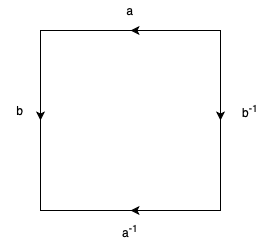
\includegraphics[scale = 0.5]{fotos_topo_2/c/c1.png}
    \end{equation}
    Aleshores escullo el vèrtex de dalt a l'esquerra com a 1 i vaig fent fletxes vermelles amb els vèrtexs amb els quals s'identifica
    \begin{equation}
        \notag
        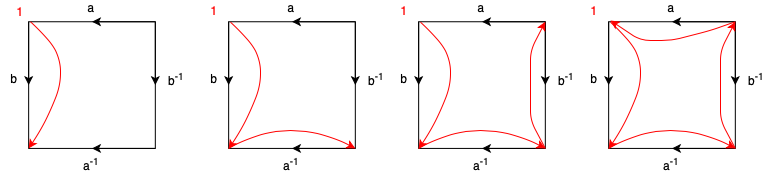
\includegraphics[scale = 0.5]{fotos_topo_2/c/c2.png}
    \end{equation}
    i finalment el resultat seria que tots els vèrtexs s'identifiquen en un sol punt.
    
    \item El mètode que és més còmode per calcular això consistirà a fer-ho de forma analítica. Si tenim una paraula $A$ anirem posant subíndexs que indicaran el vèrtex que s'identifica. Per exemple, si tenim la paraula $abcb^{-1}c^{-1}a$, posarem un subíndex allà on vulguem i anirem fent les connexions:
    \begin{equation}
        \notag
        a_1bcb^{-1}c^{-1}a\rightarrow a_1bcb^{-1}_1c^{-1}a_1 \rightarrow a_1bc_1b^{-1}_1c^{-1}a_1 \rightarrow
    \end{equation}
    \begin{equation}
        \notag
         a_1b_1c_1b^{-1}_1c^{-1}a_1 \rightarrow a_1b_1c_1b^{-1}_1c^{-1}_1a_1 \rightarrow
        _1a_1b_1c_1b^{-1}_1c^{-1}_1a_1
    \end{equation}
\end{enumerate}

\begin{ej}
Sigui $S_A$ la superfície definida per la paraula
\begin{equation}
    \notag
    A = abcb^{-1}dacefef^{-1}d^{-1}
\end{equation}
formada per sis parelles de lletres. Posem com a subíndexs de cada lletra de $A$ els vèrtexs del graf $G_A$ que resulten de realitzar les identificacions en el polígon $P_A$. Tenim així
\begin{equation}
    \notag
    _1a_1b_1c_1b^{-1}_1d_1a_1c_1e_1f_1e_1f^{-1}_1d^{-1}_1,
\end{equation}
i per tant el graf $G_A$ té només un vèrtex, en el qual s'identifiquen tots els vèrtexs de $P_A$. Així, $G_A$ és en realitat una d'aquelles floretes, que representen 6 circumferències unides en un punt. Així, $\pi(G_A)\cong F_6$, i 
\begin{equation}
    \notag
    \pi(S_A)\cong \langle a,b,c,d,e,f\;:\;abcb^{-1}dacefef^{-1}d^{-1}\rangle
\end{equation}
\end{ej}

Observem que, en particular, les paraules estàndards (\ref{def:superficieestandard}) identifiquen també tots els vèrtexs de $P_A$ en un sol punt i, per tant, es té el següent resultat.
\begin{coro}
Si $S_A$ és una superfície compacta, connexa i definida per la paraula estàndard $A$, aleshores
\begin{enumerate}
    \item Si $A = A_g$, llavors $\pi(S_A)\cong\langle a_1,b_1,\ldots,a_n,b_n\;:\;A_g\rangle$.
    \item Si $A = B_g$, llavors $\pi(S_A)\cong\langle a_1,b_1,\ldots,a_n,b_n\;:\;B_g\rangle$
\end{enumerate}
\end{coro}


\subsection{El cas general}

En el cas general els vèrtexs del polígon $P_A$ no s'identifiquen en un sol punt, sinó que s'identifiquen donant $v'\geq 1$ punts diferents, que seran els vèrtexs del graf $G_A$. Així, el graf $G_A$ ja no serà una floreta de circumferències, però això no és un problema ja que sabem quin és el grup fonamental d'un graf connex qualsevol (vist a \ref{ter:numerodebetti}), doncs vam veure que un graf connex $G$ amb $v$ vèrtexs i $a$ arestes era homotòpicament equivalent a la unió puntual de $\ell = 1-v+a$ circumferències i, per tant, $\pi(G)\cong F_\ell$.

Recordem la demostració del teorema (\ref{ter:numerodebetti}) ja que d'ella se seguirà el següent teorema. Per inducció sobre el nombre de vèrtexs $v$ fèiem que si $G$ tenia un sol vèrtex, i.e. $v=1$, $G$ era la unió puntual de $a$ circumferències i per tant $\pi(G)\cong F_a$, cosa que prova el teorema en aquest cas. Si, en canvi, teníem més d'un vèrtex, existirà una aresta entre vèrtexs diferents, doncs $G$ és connex. Si contraiem aquesta aresta a un punt, s'obté un nou graf $G'$ amb $v'=v-1$ vèrtexs i $a'=a-1$ arestes. Per hipòtesi d'inducció $\pi(G')\cong F_{\ell'}$, essent $\ell' = 1-v'+a'$. Però com $\ell' = 1-v'+a'=1-v+1+a-1=1-v+a=\ell$, i $G'$ és del mateix tipus d'homotopia que $G$, podem concloure que $\pi(G)\cong \pi(G')\cong F_\ell$, com volíem.

\begin{ter}
\label{ter:grupdelgrafgeneral} Amb les hipòtesis anteriors, si $\alpha_1,\ldots,\alpha_a$ són les arestes de $G$ i es contrauen $\alpha_{\ell+1},\ldots,\alpha_a$ per obtenir $G'$ un graf amb només un vèrtex, aleshores $\pi(G)$ és el grup lliure de generadors $\alpha_1,\ldots,\alpha_\ell$, que són les imatges de les arestes en $\pi(G')$ que no s'han contret. És a dir,
\begin{equation}
    \notag
    \pi(G)\cong\langle \alpha_1,\ldots,\alpha_\ell\;\rangle.
\end{equation}
A més, si $\alpha$ és un llaç en $G$ determinat per una paraula en les arestes de $G$ com a parella de lletres, la seva imatge en $\pi(G)$ és una paraula amb $\ell$ parelles de lletres.
\end{ter}
\begin{proof}
Com en l'anterior demostració, se segueix fàcilment per inducció sobre el número de vèrtexs $v$ de $G$.
\end{proof}

Tornant al graf $G_A$ de la superfície $S_A$, com $G_A$ és un graf amb $n$ arestes i $v'$ vèrtexs resulta que
\begin{ter}
\label{ter:teoremagraf4} Si els vèrtexs del polígon $P_A$ s'identifiquen donant $v'$ punts diferents, aleshores
\begin{equation}
    \notag
    \pi(S_A)\cong\langle \alpha_1,\ldots,\alpha_r\;:\;A'\rangle
\end{equation}
essent $r = 1-v'+n$, $\alpha_1,\ldots,\alpha_r$ les imatges de les arestes $\alpha_1,\ldots,\alpha_r$ de $G_A$ que no s'han contret al contraure les arestes necessàries per convertir $G_A$ en un graf amb un sol vèrtex, i $A'$ la paraula amb $r$ parelles de lletres que resulta de $A$.
\end{ter}

\begin{ej}
Sigui $S_A$ la superfície definida per la paraula $abca^{-1}defbec^{-1}d^{-1}f$. Si posem com a subíndexs de cada lletra d'$A$ els vèrtexs del graf $G_A$ que resulten de realitzar les identificacions en el polígon $P_A$, es té
\begin{equation}
    \notag
    _1a_1b_2c_1a_1^{-1}d_2e_1f_1b_2e_1c^{-1}_2d^{-1}_1f_1
\end{equation}
i per tant $v'=2$. Així, $r = 1-2+6=5$ i per tant $\pi(G_A)\cong F_5$.
\end{ej}

\subsection{Orientabilitat}

Podem donar una primera definició d'orientabilitat d'una superfície definida per una paraula a partir de la propia paraula com següeix.

\begin{defi}
[Heterotipus i homotipus]\label{def:heterotipus}\label{def:homotipus} Una parella de lletres $a,a^{\pm 1}$ d'una paraula $A$ direm que és una parella \textit{heterotipus}\index{Heterotipus} (o de primer tipus) si en $A$ apareixen $a$ i $a^{-1}$. En canvi direm que és una parella \textit{homotipus}\index{Homotipus} (o de segon tipus) si en $A$ figuren $a$ i $a$.
\end{defi}

\begin{defi}
[Orientable]\label{def:orientable}\index{Orientable}\index{Superfície orientable} Sigui $S_A$ una superfície compacta, connexa i definida per una paraula $A$. Direm que $S_A$ és una superfície \textit{orientable} si totes les parelles de $A$ són heterotipus. En cas contrari, és a dir, si existeix una parella homotipus a $A$, direm que $S_A$ és \textit{no orientable}.
\end{defi}

\begin{ej}
Les paraules estàndards $A_g$ tenen totes les seves parelles de lletres de primer tipus i, per tant, defineixen superfícies orientables. D'altra banda, les paraules estàndards $B_g$ tenen totes les seves parelles de lletres de segon tipus i, per tant, defineixen superfícies no orientables.
\end{ej}

L'abelianització d'un grup $G$ és el quocient del grup $G$ per la relació $ab=ba$. Es denota per $G_{ab}$.

\begin{ter}
\label{ter:grupfonamentalsuperficieorientable} Sigui $S_A$ una superfície compacta, connexa i definida per la paraula $A$. Aleshores:
\begin{enumerate}[(a)]
    \item $S_A$ és orientable si, i només si, $\pi(S_A)_{ab}\cong \mathbb{Z}^{2g}$, i
    \item $S_A$ és no orientable si, i només si, $\pi(S_A)_{ab}\cong\mathbb{Z}^{g-1}\oplus \mathbb{Z}/2\mathbb{Z}$
\end{enumerate}
\end{ter}
\begin{proof}
Es deixa com a exercici donar una prova directa d'aquest resultat ja que, més endavant, obtindrem una prova immediat com a conseqüència del Teorema de Classificació (\ref{ter:classificaciosuperficies}) que veurem més endavant.
\end{proof}

Amb la definició d'orientabilitat que hem donat en (\ref{def:orientable}) podria passar que dues superfícies homeomorfes fossin una orientable i l'altra no, depenent de la paraula que les defineix. El corol·lari que segueix establirà la invariància topològica de l'orientabilitat i demostra, doncs, que no és així.

\begin{coro}
\label{coro:orientabilitatesuninvarianttopologic} L'orientabilitat és un invariant topològic\footnote{Recordem la definició de invariant topològic dels apunts de Topologia.}. És a dir, siguin $S_A$ i $S_B$ dues superfícies homeomorfes definides per les paraules $A$ i $B$ respectivament. Llavors $S_A$ és orientable si, i només si, $S_B$ és orientable.
\end{coro}
\begin{proof}
Resulta del teorema anterior, ja que les superfícies orientables no tenen elements de torsió en el seu grup fonamental abelianitzat, mentre que les no orientables sí que tenen torsió\footnote{Recordem (no sé d'on perquè jo això no ho havia sentit mai) que si $p$ és un nombre natural positiu i $g$ és un element d'un grup abelià $G$, llavors es diu que és de $p$-torsió si $pg=0$.} (2-torsió per ser més precisos) en el seu grup fonamental abelianitzat.
\end{proof}


\section{Classificació de superfícies}

En les properes subseccions es buscarà provar el teorema de classificació de superfícies (\ref{ter:classificaciosuperficies}) i per això es provaran una sèrie de resultats. Aquest teorema servirà per classificar les superfícies poligonals $S_A$ a partir de la paraula $A$ que la defineix.

Abans, però, cal fer un petit incís en la notació utilitzada. Quan posem $gX$, on $X$ és una superfície qualsevol i $g$ és un enter positiu qualsevol, ens referim a la paraula que genera $g$ superfícies $X$. Per exemple, $2T^2$ seria $aba^{-1}b^{-1}cdc^{-1}d^{-1}$.

\begin{ter}
[Classificació de superfícies]\label{ter:classificaciosuperficies}\index{Teorema de classificació de superfícies} Sigui $A$ una paraula de $n$ parelles de lletres tal que, al identificar-se les parelles de costats de $P_A$ que determina la paraula $A$, el graf $G_A=\partial P_A/\sim$ resultant té $v'$ vèrtexs. Llavors
\begin{itemize}
    \item Si totes les parelles de $A$ són heterotipus, $S_A\cong g\mathbb{T}^2$, amb $g = \frac{1}{2}(1-v'+n)$;
    \item Si en $A$ hi ha una parella homotipus, $S_A\cong g\mathbb{R}P^2$, amb $g=1-v'+n$.
\end{itemize}
A l'enter $g\geq 0$ se li diu \textit{gènere} de la superfície $S_A$.
\end{ter}

\begin{ej}
Considerem la superfície $S_A$ generada per la paraula
\begin{equation}
    \notag
    A=abca^{-1}defbec^{-1}d^{-1}
\end{equation}
Com la parella $bb$ és homotipus, la superfície $S_A$ serà no orientable. Si posem com a subíndexs de cada lletra de $A$ els vèrtexs del graf $G_A$ que resulten al realitzar les identificacions en el polígon $P_A$, es té 
\begin{equation}
    \notag
    _1a_1b_2c_1a^{-1}_1d_2e_1f_1b_2e_1c^{-1}_2d^{-1}_1f_1
\end{equation}
i per tant $v'=2$. Així, el gènere de $S_A$ és 
\begin{equation}
    \notag
    g=1-v'+n=1-2+6=5
\end{equation}
Per tant es conclou que $S_A\cong 5\mathbb{R}P^2$
\end{ej}

\subsection{Demostració del teorema de classificació de superfícies}

Denotarem $\mathcal{A} = \{a_1,a_1^{- 1},b_1,b_1^{-1},\ldots\}$ el conjunt de lletres amb les quals formem les paraules que defineixen superfícies compactes, connexes, i.e. paraules amb només parells de lletres. Designarem per lletres minúscules un element arbitrari de $\mathcal{A}$.

\begin{ter}
[Riemann, Veblen, 1915]\label{ter:riemannsuperficiesparaules} Tota superfície compacta, connexa i definida per una paraula és homeomorfa a una única superfície estàndard.

Més precisament, sigui $S_A$ la superfície definida per la paraula $A$ amb parelles de lletres. Aleshores
\begin{enumerate}[(i)]
    \item Si totes les parelles de $A$ són heterotipus, $S_A\simeq S_{A_0}$, o bé $S_A\simeq S_{A_g}$;
    \item Si en $A$ existeix alguna parella homotipus, $S_A\simeq S_{B_g}$
\end{enumerate}
\end{ter}
Abans de poder començar amb la prova d'aquest teorema caldran unes consideracions prèvies que permetran ``algebraitzar'' el problema.

Designarem per $\mathcal{W}$ el conjunt de les paraules amb només parelles de lletres, i.e. aquelles que defineixen superfícies compactes i connexes, i per lletres majúscules $A,B,C,\ldots$, les paraules de $\mathcal{W}$. Designarem amb les lletres majúscules $X,Y,Z,\ldots$, subparaules de les anteriors, i.e. amb parelles de lletres i/o lletres d'una sola paraula buida.

En $\mathcal{W}$ considerem la relació d'equivalència $\sim$ generada per les relacions:
\begin{enumerate}[(i)]
    \item $A\sim B$ si $B$ s'obté a partir de $A$ ``reanomenant'' les lletres que formen $A$, és a dir, a partir d'una bijecció $\mathcal{W}\rightarrow \mathcal{W}$ que conserva els inversos
    \item $A=aX\sim B=Xa$, és a dir, les paraules que són cíclicament iguals són equivalents.
    \item $A = XaYUa^{\pm 1}V\sim B=bU(X^{-1}bY^{-1})^{\pm 1}V$, que correspon al ``canvi de variable'' $XaY=b$.
    \item $aa^{-1}B\sim B$.
    \item $AC\sim BC$ si $A\sim B$.
\end{enumerate}

\begin{lema}
[De l'àlgebra a la topologia]\label{lema:delalgebraalatopologia} Si dues paraules $A$ i $B$ de $\mathcal{W}$ són equivalents, les superfícies que defineixen són homeomorfes, és a dir, $A\sim B$ implica que $S_A\simeq S_B$.
\end{lema}
\begin{proof}
En efecte, donat que la relació d'homeomorfisme és una relació d'equivalència, serà suficient que provem el lema per a cadascuna de les relacions que generen $\sim$.
\begin{enumerate}[(i)]
    \item Si $B$ s'obté a partir d'$A$ reanomenant les lletres que defineixen $A$, les identificacions de costats que defineixen $A$ i $B$ són les mateixes.
    \item Les paraules $aX$ i $Xa$ defineixen superfícies homeomorfes, ja que només es diferencien en el vèrtex del polígon a partir del qual es comença la paraula que indica les identificacions dels costats.
    \item Si $A= XaYUa^{\pm1}V$ i $B=bU(X^{-1}bY^{-1})^{\pm 1}V$, les superfícies $S_A$ i $S_B$ són homeomorfes, doncs si es talla la regió poligonal $P_A$ pel segment $b$ que uneix l'origen de $X$ amb l'extrem de $Y$, s'obtenen dues regions poligonals marcades, cadascuna d'elles amb un costat $a$ i un costat $b$. Si primer s'identifiquen els costats $b$ i després els altres costats s'obté la superfície original $S_A$, però si primer s'identifiquen els costats $a$ i després els altres costats s'obté $S_B$. Com la superfície final no depèn, tret d'homeomorfisme, de l'ordre en què s'hagin fet les identificacions, es conclou que $S_A\simeq S_B$.
    \item Si $A=aa^{-1}B$, es té que $S_A\simeq S_B$, ja que al identificar $a$ amb $a^{-1}$ s'obté un polígon amb dos costats menys i amb la paraula $B$:
    \begin{equation}
        \notag
        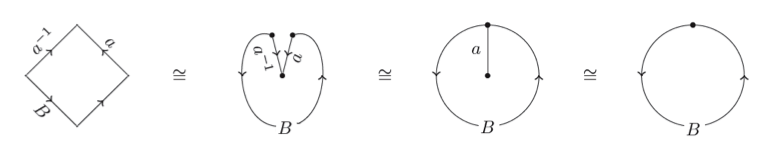
\includegraphics[scale = 0.5]{fotos_topo_2/delalgbraalatopologia.png}
    \end{equation}
    Observem que aquesta relació elimina l'esfera $aa^{-1}$ i és l'expressió algebraica que l'esfera és l'element neutre de la suma connexa, i.e. $S^2\#S_B\simeq S_B$.
    \item Finalment, per inducció sobre la longitud de les paraules, podem suposar que $A\sim B$ implica que $S_A\simeq S_B$ i com que $S_{AC}\simeq S_A\#S_C$ i $S_{BC}\simeq S_B\#S_C$, se segueix que $S_{AC}\simeq S_{BC}$.
\end{enumerate}
\end{proof}

\begin{lema}[Creació de plans projectius]
\label{lema:creaciodeplansprojectius} Si $A = aXaY$, llavors $A\sim bbB$, amb $B=X^{-1}Y$
\end{lema}
\begin{proof}
És suficient fer $aX=b$, ja que aleshores $a=bX^{-1}$ i així $A=aXaY\sim bbX^{-1}Y = bbB$.
\end{proof}

\begin{lema}\label{lema:lema3}
$B_1A_1=aabcb^{-1}c^{-1}\sim B_3=ddeeff$.
\end{lema}
\begin{proof}
En efecte, fent $d = abcb^{-1}$ s'obté que $a = dbc^{-1}b^{-1}$, i per tant $aabcb^{-1}c^{-1}\sim dbc^{-1}b^{-1}dc^{-1}$. Fent $f = b^{-1}dc^{-1}$ s'obté que $c^{-1}=d^{-1}bf$, i resulta que $aabcb^{-1}c^{-1}\sim dbd^{-1}bff$. Finalment, fem $e = d^{-1}b$, $b=de$ i resulta $abcb^{-1}c^{-1}\sim ddeeff$.
\end{proof}

\begin{lema}
[Creació de torus]\label{lema:creaciodetorus} Si $A = aXbYa^{-1}Ub^{-1}V$, llavors $A\sim cdc^{-1}d^{-1}B$, amb $B=XVUY$.
\end{lema}
\begin{proof}
En efecte, primer es fa $XbY=d$, i aleshores $b= X^{-1}dY^{-1}$, $b^{-1}=Yd^{-1}X$, i així
\begin{equation}
    \notag
    A=aXbYa^{-1}Ub^{-1}V\sim ada^{-1}UYd^{-1}XV
\end{equation}
i després es fa $c^{-1}=a^{-1}UY$, doncs així $a = UYc$, i resulta finalment
\begin{equation}
    \notag
    A\sim UYcdc^{-1}d^{-1}XV\sim cdc^{-1}d^{-1}XVUY=cdc^{-1}d^{-1}B
\end{equation}
\end{proof}

Amb aquests preliminars podem ja abordar la prova del teorema (\ref{ter:riemannsuperficiesparaules}).

\begin{proof}
[del teorema \ref{ter:riemannsuperficiesparaules}] Sigui $S_A$ la superfície definida per la paraula $A$ de $n$ parelles de lletres. Pel lema (\ref{lema:delalgebraalatopologia}), per provar que $S_A$ és homeomorfa a una superfície estàndard, serà suficient provar que $A$ és equivalent a una paraula estàndard. La prova la farem per inducció sobre $n$.

Si $n=1$, aleshores $A = aa^{-1}$ o bé $A = aa$ i per tant el teorema està demostrat en aquest cas. Suposem que $n>1$ i tractarem el cas orientable i el no orientable per separat.
\begin{enumerate}[(a)]
    \item Si en $A$ hi ha una parella homo, per (ii) serà $A\sim aXaY$ i pel lema (\ref{lema:creaciodeplansprojectius}) $A\sim bbB$, amb $B = X^{-1}Y$. Utilitzant ara la hipòtesi d'inducció i (v), podem concloure que $A\sim bbB\sim bbB_{g-1}\sim B_g$, o bé que $A\sim bbB\sim B_1A_{g-1}$ i, en aquest últim cas, aplicant reiteradament el lema (\ref{lema:lema3}) podem concloure que també $A\sim B_g$.
    \item Si totes les parelles de $A$ són hetero, considerem la parella $a$, $a^{-1}$, que estigui mínimament separada, i.e. que hi hagi entre mig el menor número $s$ de lletres, considerada $A$ com una paraula cíclica, i.e. considerant $A$ i totes les paraules cíclicament equivalents. Si $s=0$, aplicant reiteradament la relació (ii), tindrem que $A\sim aa^{-1}B$ i, per (iv), $A\sim B$. Com $B$ té també totes les seves parelles hetero i té $2n-2$ lletres, $B\sim A_g$ per la hipòtesi d'inducció, i en conseqüència, $A\sim A_g$. Si $s>0$, direm que $A$ té dues parelles hetero enllaçades i aplicant (ii) tindrem que $A\sim aXbYa^{-1}Ub^{-1}V$ i es té que pel lema (\ref{lema:creaciodetorus}) $A\sim UYcdc^{-1}d^{-1}XV\sim cdc^{-1}d^{-1}XVUY\sim cdc^{-1}d^{-1}B$.
    
    Com $B = XVUY$, i totes les parelles de $A$ eren hetero, també totes les parelles de $B$ són hetero. Així, aplicant de nou la hipòtesi d'inducció, concloem que $B\sim A_{g-1}$ i, per (v), $cdc^{-1}d^{-1}B\sim cdc^{-1}d^{-1}A_{g-1}$. Per tant, es té que
    \begin{equation}
        \notag
        A\sim cdc^{-1}d^{-1}B\sim cdc^{-1}d^{-1}A_{g-1}\sim A_g.
    \end{equation}
    
    En definitiva, hem demostrat que la paraula $A$ és equivalent a una paraula estàndard. Ara, la unicitat de la superfície estàndard homeomorfa a $S_A$ es dedueix del càlcul dels subgrups fundamentals abelianitzats de les superfícies estàndards:
    \begin{equation}
        \notag
        \pi(S^2)_{ab}\cong 0,\quad \pi(g\mathbb{T}^2)_{ab}\cong\mathbb{Z}^{2g},\quad \pi(g\mathbb{R}P^2)_{ab}\cong \mathbb{Z}^{g-1}\oplus\mathbb{Z}/2\mathbb{Z}.
    \end{equation}
    ja que aquests grups no són isomorfs dos a dos i, per tant, aquestes superfícies no són homeomorfes dues a dues.
\end{enumerate}
\end{proof}

\begin{coro}
\label{coro:orientable1} Dues superfícies compactes, connexes i definides per paraules són homeomorfes si, i només si, els seus grups fonamentals són isomorfs.
\end{coro}

\begin{coro}
\label{coro:orientable2} Sigui $S_A$ una superfície compacta, connexa i definida per una paraula $A$. Aleshores, 
\begin{itemize}
    \item $S_A$ és orientable si, i només si, $\pi(S_A)_{ab}\cong \mathbb{Z}^{2g}$;
    \item $S_A$ és no orientable si, i només si $\pi(S_A)_{ab}\cong \mathbb{Z}^{g-1}\oplus\mathbb{Z}/2\mathbb{Z}$.
\end{itemize}
\end{coro}























\section{Triangulació}

A partir d'ara totes les superfícies seran compactes, connexes i sense vora.


\subsection{Superfícies triangulables}

\begin{defi}
[Triangle estàndard]\label{def:triangleestandard}\index{Triangle estàndard} Denotem $\Delta := \{(x,y)\in\mathbb{R}^2\;:\;x\geq 0,\;y\geq 0,\;x+y\geq 1\}\subseteq \mathbb{R}^2$. Si ens hi fixem, veiem que $\Delta$ és un triangle ``ple'', l'anomenarem \textit{triangle estàndard}.
\end{defi}

\begin{defi}
[Triangle en una superfície]\label{def:triangleens}\index{Triangle en una superfície}\index{Triangle en $S$} Sigui $S$ una superfície, un \textit{triangle en $S$} és un tancat $T\subseteq S$ tal que existeix un homeomorfisme $\varphi:\Delta\rightarrow T$. Les imatges per $\varphi$ dels costats i dels vèrtex de $\Delta$ els anomenarem costats i vèrtex de $T$.
\end{defi}

\begin{defi}
[Triangulació d'una superfície]\label{def:triangulacio}\index{Triangulació d'una superfície} Una triangulació $\mathcal{T}$ de $S$ és una família de triangles $\mathcal{T}=\{T_i\}_{i\in I}$ en $S$, tals que
\begin{enumerate}[(i)]
    \item $S = \bigcup_{i\in I}T_i$
    \item Si $T_i\cap T_j\not=\emptyset$ per $i\not=j$ aleshores $T_i\cap T_j$ és un vèrtex de $T_i$ i de $T_j$ o bé un costat de $T_i$ i $T_j$.
\end{enumerate}
\end{defi}

\begin{ej}
\label{ej:exemplesdetriangles} Les següents interseccions de dos triangles sí que compleixen les condicions per ser una triangulació ja que al primer cas la intersecció és un vèrtex i al segon cas una aresta comuna:
\begin{equation}
    \notag
    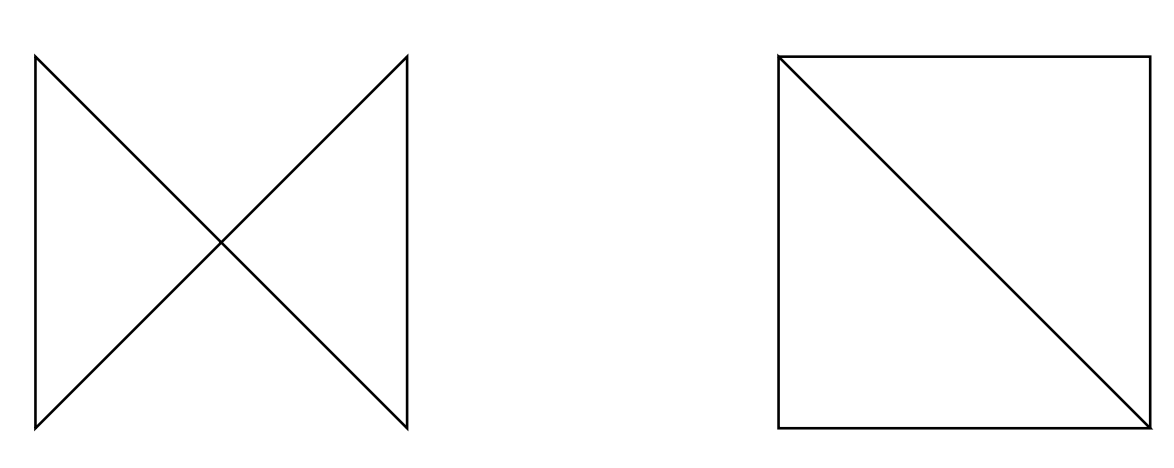
\includegraphics[scale = 0.5]{fotos_topo_2/triangulacioricardo/t1.png}
\end{equation}
En canvi, la següent intersecció no compleix les condicions per ser una triangulació ja que la seva intersecció no és ni una aresta ni un vèrtex comú:
\begin{equation}
    \notag
    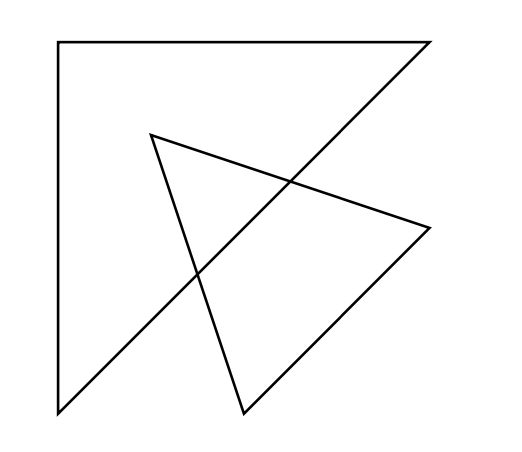
\includegraphics[scale = 0.5]{fotos_topo_2/triangulacioricardo/t2.png}
\end{equation}
\end{ej}

\begin{ej}
\label{ej:triangulaciotorus} Ens podem preguntar si el torus és una superfície triangulable. Per exemple, la següent figura podria ser una triangulació del tor?
\begin{equation}
    \notag
    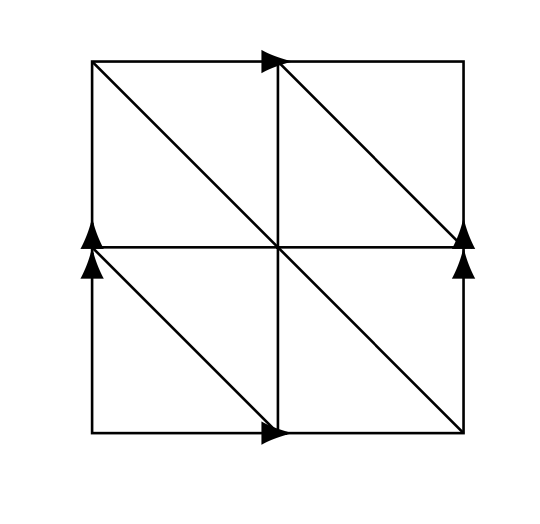
\includegraphics[scale = 0.5]{fotos_topo_2/triangulacioricardo/t3.png}
\end{equation}
Aquesta descomposició no és una triangulació del tor, observem aquests dos triangles:
\begin{equation}
    \notag
    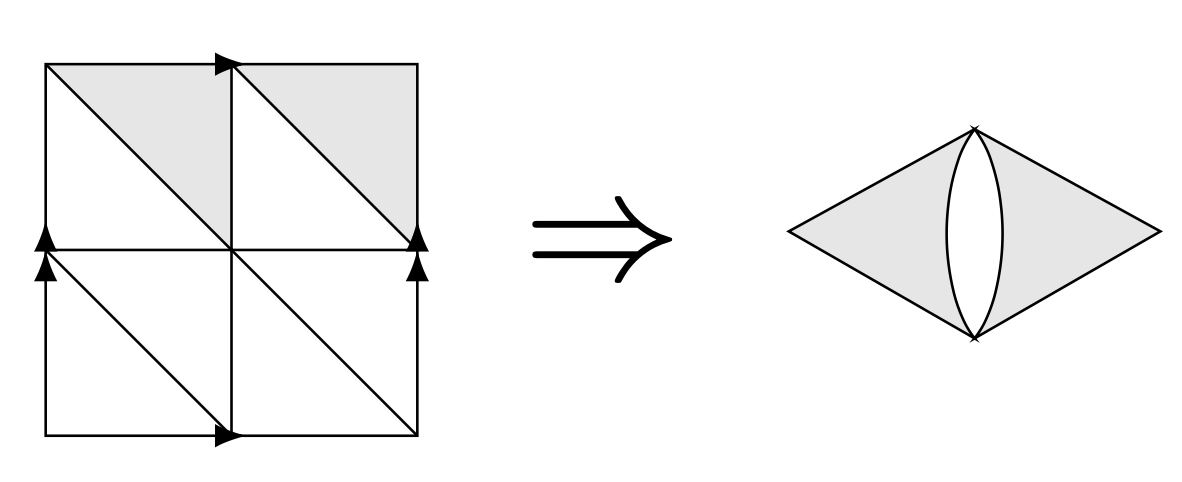
\includegraphics[scale = 0.5]{fotos_topo_2/triangulacioricardo/t4.png}
\end{equation}
Com que els costats estan identificats, veiem que s'intersequen en dos punts, que són dos vèrtexs, però no tenen cap aresta en comú. Per tant, com que la seva intersecció no és ni un únic vèrtex ni tampoc cap aresta, veiem que aquests triangles no formen cap triangulació del tor. 

En canvi, els següents triangles sí que formen una triangulació del tor:
\begin{equation}
    \notag
    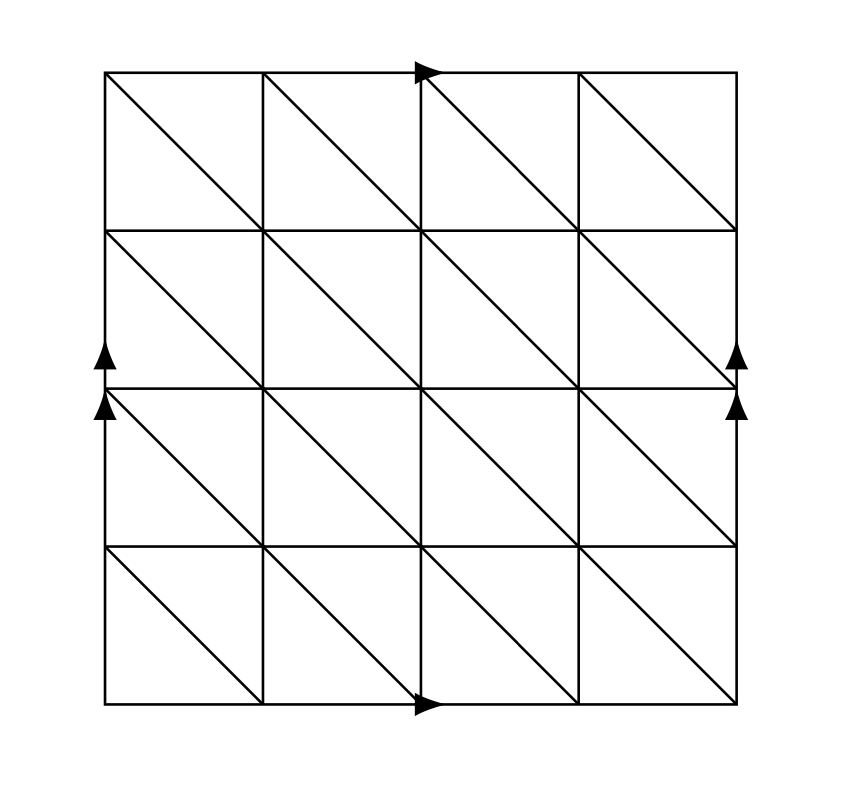
\includegraphics[scale = 0.5]{fotos_topo_2/triangulacioricardo/t5.png}
\end{equation}
\end{ej}

\begin{nota}
\label{nota:triangulaciosuperficies} També ens podem preguntar si, en general, les superfícies poligonals són triangulables. La resposta és afirmativa. Donada una superfície poligonal, primer de tot agafem el centre del polígon regular (el centre de la circumferència circumscrita) i des de cada vèrtex del polígon l'unim al centre amb un segment. Ens quedarà una divisió del polígon en triangles, però aquesta divisió no serà una triangulació.
\begin{equation}
    \notag
    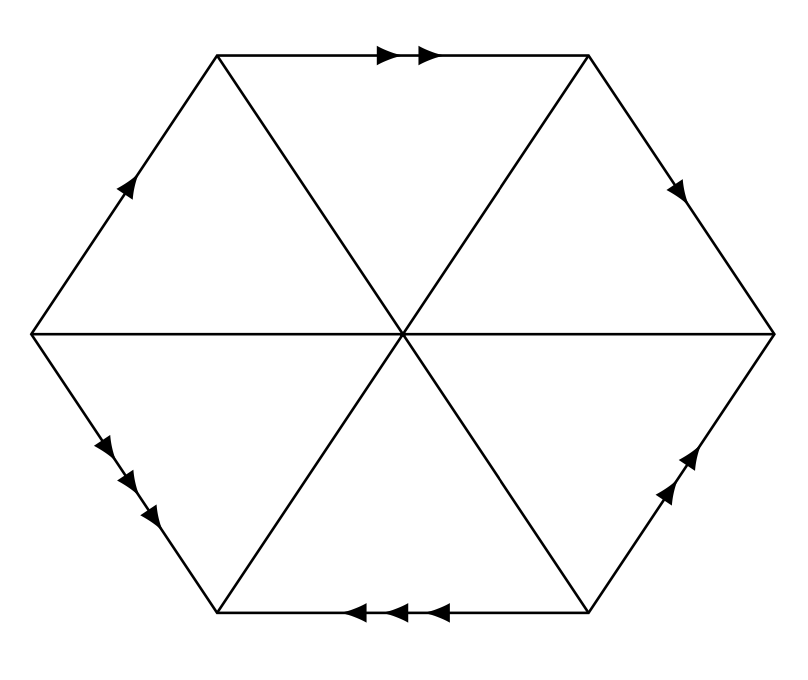
\includegraphics[scale = 0.5]{fotos_topo_2/triangulacioricardo/t6.png}
\end{equation}
És molt fàcil veure que no és cap triangulació ja que si agafem dos triangles que tinguin els costats ``exteriors'' identificats, aleshores la seva intersecció és un vèrtex i una aresta, i el vèrtex no és un extrem de l'aresta.

El que hem de fer és subdividir cadascun d'aquests triangles, per exemple, de la següent manera:
\begin{equation}
    \notag
    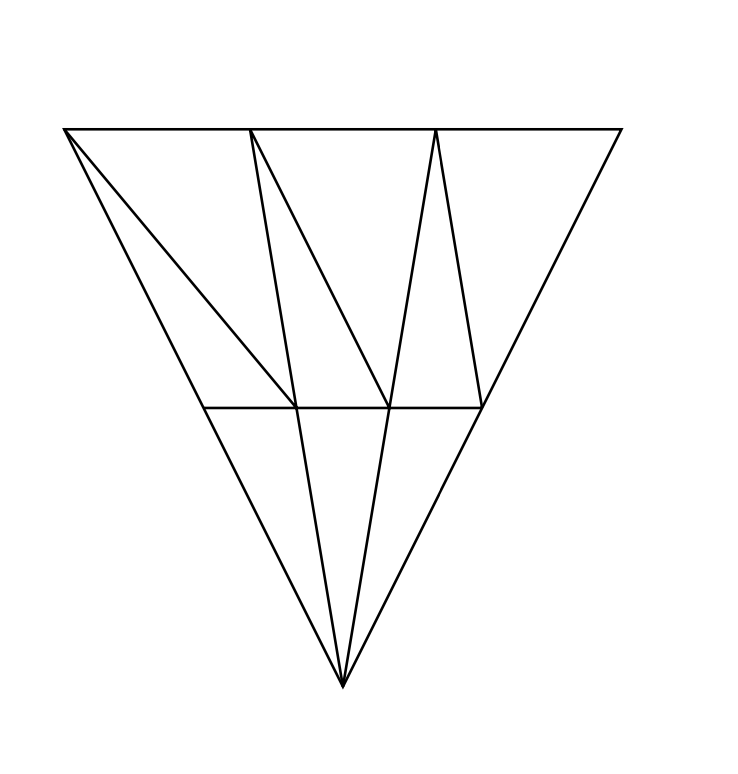
\includegraphics[scale = 0.5]{fotos_topo_2/triangulacioricardo/t7.png}
\end{equation}
Ara, però, cal formalitzar tot això.
\end{nota}

\begin{prop}
[Triangulació de superfícies]\label{prop:triangulaciosuperficies} Tota superfície compacta connexa $S_A$ definida per una paraula $A$ amb $n$ parelles de lletres és triangulable.
\end{prop}
\begin{proof}
Com que $S_A\simeq P/\sim_A$, on $P$ és el polígon de $2n$ costats regular, és suficient observar que la triangulació de $P$ obtinguda al triangular cadascun dels seus $2n$ ``triangles centrals'' de $P$ com s'ha fet a l'observació anterior (\ref{nota:triangulaciosuperficies}) indueix una triangulació en $S_A$.
\end{proof}

Encara es pot provar més:
\begin{ter}
\label{ter:totasuperficiecompactaestriangulable} Tota superfície compacta $M$ és triangulable.
\end{ter}
\begin{proof}
Una manera de demostrar això és escollir, per a cada punt $p\in M$, una carta local $(U_p,\varphi_p)$ amb $p\in U_p$ i escollir un disc tancat $D_p\subset \varphi_p(U_p)$ de centre $\varphi_p(p)$. Llavors els oberts $V_p = (\varphi_p)^{-1}(D_p^\circ)$ recobreixen $M$. Com que $M$ és compacta, podem escollir un nombre finit de punts $p_1,\ldots,p_n$ tals que $V_{p_1},\ldots,V_{p_n}$ recobreixin $M$. Les vores $\partial\overline{V}_{p_1},\ldots,\partial\overline{V}_{p_n}$ formen un graf a $M$ que es pot refinar a una triangulació després de rectificar els arcs que calguin per tal que cada intersecció $\partial\overline{V}_{p_i}\cap \partial\overline{V}_{p_j}$ sigui un conjunt finit de punts.
\end{proof}

Per tal de detallar com es poden ``rectificar els arcs que calguin'', és necessari utilitzar el fet que tota corba tancada simple a $\mathbb{R}^2$ delimita dues regions, una de les quals és homeomorfa a un disc obert. Aquest fet, malgrat que sembli evident, no és gens senzill de demostrar. Es dedueix del \textit{teorema de Jordan-Schönflies} que només enunciarem i comentarem a continuació.

\begin{defi}
[Corba de Jordan]\label{def:corbadejordan}\index{Corba de Jordan} Una \textit{corba tancada simple}\index{Corba tancada simple} o \textit{corba de Jordan} és un subespai de $\mathbb{R}^2$ homeomorf a la circumferència $S^1$.
\end{defi}

\begin{ter}
[Teorema de Jordan]\label{ter:teoremadejordan}\index{Teorema de Jordan} Si $C$ és una corba de Jordan, llavors $\mathbb{R}^2\setminus C$ té dues components connexes, una de les quals és acotada i l'altra no ho és. A més, $C$ és la frontera de cadascuna d'aquestes dues components. 
\end{ter}
\begin{proof}
No demostrarem aquest resultat perquè utilitza eines que no hem estudiat encara\footnote{La primera demostració rigorosa coneguda d'aquest resultat es troba en un llibre de Camille Jordan, publicat el 1887. El 1905, Oswald Veblen va donar-ne una altra demostració més acurada, considerada per molts la primera demostració completa i correcta. Més tard, s'han anat publicant demostracions més elementals, com les de Filippov (1950) i Thomassen (1992)}.
\end{proof}

La següent generalització del teorema de la corba de Jordan, anomenada teorema de Jordan-Brouwer \label{ter:teoremadejordanbrouwer}\index{Teorema de Jordan-Brouwer}, és vàlida en qualsevol dimensió: si $X$ és un subespai de $\mathbb{R}^{n+1}$ homeomorf a l'esfera $S^n$, on $n\geq 1$, llavors $\mathbb{R}^{n+1}\setminus X$ té dues components connexes, una de les quals és acotada i l'altra no ho és. A més, $X$ és la frontera de cadascuna d'aquestes dues components. 

Arthur Schönflies va publicar entre 1890 i 1895 diversos resultats sobre corbes tancades i simple. El fet següent, important i útil, porta el seu nom:

\begin{ter}
[Teorema de Jordan-Schönflies]\label{ter:teoremadejordanschonflies}\index{Teorema de Jordan-Schönflies}  Tota aplicació injectiva i contínua $S^1\rightarrow \mathbb{R}^2$ es pot estendre a un homeomorfisme $\mathbb{R}^2\rightarrow \mathbb{R}^2$.
\end{ter}

Aquest fet no només implica el teorema de la corba de Jordan, sinó que ens diu que, si $C$ és una corba de Jordan, llavors la component acotada de $\mathbb{R}^2\setminus C$ és homeomorfa a un disc obert i la component no acotada és homeomorfa a l'exterior d'un disc tancat.

Tanmateix, el teorema de Jordan-Schönflies no és cert en dimensions superiors. Per exemple, a l'espai $\mathbb{R}^3$ hi ha subespais homeomorfs a l'esfera $S^2$ tals que la component no acotada no és simplement connexa, com l'anomenada ``esfera amb banyes'' de James Alexander (1924).

Una demostració rigorosa del fet que les superfícies compactes són triangulables va ser descrita per Tibor Radó l'any 1925. En la dècada de 1950 Bing i Moise van demostrar que les varietats compactes de dimensió 3 també ho són. A més, en dimensions 2 i 3 cada triangulació és única, llevat d'equivalència. No obstant, en dimensió 4 hi ha varietats compactes que no són triangulables (Freedman, 1980) i d'altres que admeten infinites triangulacions no equivalents (Donaldson, 1987). L'any 2013, Ciprian Manolescu va demostrar que en tota dimensió superior a 4 hi ha varietats compactes no triangulables. Tanmateix, totes les varietats \textit{diferenciables} admeten triangulacions. 

\subsection{Triangulació de superfícies}



En aquesta secció, demostrarem el teorema que afirma que tota superfície compacta i connexa és triangulable si, i només si, és homeomorfa a una superfície definida per una paraula de $n$ parelles de lletres. Abans, però, escriuré un parell de resultats ja que seran necessaris per a la demostració del esmentat teorema.

\begin{prop}
\label{prop:triangulacio1} Sigui $S$ una superfície compacta i connexa, i sigui $\mathcal{T} = \{T_i\}_{i\in I}$ una triangulació finita de $S$, amb $N$ triangles. Aleshores, existeix:
\begin{itemize}
    \item Un polígon pla $P_N$ de $N+2$ costats, regular, amb una triangulació per diagonals internes (i.e. sense cap altres vèrtexs que els de $P_N$); $\mathcal{T}_N=\{W_{N,i}\}_{i=1,\ldots,N}$ amb $N$ triangles.
    \item Una aplicació contínua $\varphi_N:P_N\rightarrow S$, que indueix un homeomorfisme $W_{N,i}\rightarrow T_i$ entre els triangles de $\mathcal{T}_N$ i $\mathcal{T}$.
    \item Una paraula $A$ de parelles de lletres, tal que $\varphi_N$ indueix un homeomorfisme $P_N/\sim_A\simeq S$.
\end{itemize}
\end{prop}
\begin{proof}
Aquest resultat és conseqüència directa del següent lema (\ref{lema:triangulacio1}).
\end{proof}

\begin{lema}
\label{lema:triangulacio1} Sigui $T_1$ un triangle de $\mathcal{T}$. Aleshores existeix una successió creixen de subespais tancats de $S$, $R_1\subseteq R_2\subset\cdots\subset R_N$ tal que
\begin{itemize}
    \item $R_1 = T_1$ i $R_N=S$,
    \item Per cada $n$ tal que $1\leq n \leq N$, es té $R_n = R_{n-1}\cup T_n$, essent $T_n$ un triangle de $\mathcal{T}$ no contingut en $R_{n-1}$, i tal que $R_{n-1}\cap T_n$ conté una aresta de $T_n$.
    \item Per a cada $n$ tal que $1\leq n\leq N$, la frontera de $R_n$ és una reunió no buida d'arestes de triangles de $\mathcal{T}$.
    \item Per a cada $n$ tal que $1\leq n\leq N$, existeix un polígon pla $P_n$ de $n+2$ costats, regular, amb una triangulació $\mathcal{T}_n = \{W_{n,i}\}_{i=1,\ldots,n}$ per diagonals internes (i.e. sense altres vèrtexs que els de $P_n$), i una aplicació contínua $\varphi_n:P_n\rightarrow R_n$, que indueix homeomorfismes $W_{n,i}\rightarrow T_i$ entre els triangles de $\mathcal{T}_n$ i els de $R_n$, i la restricció de la qual a l'interior de $P_n$ és un homeomorfisme sobre la seva imatge.
    \item Existeix una paraula $A$ de parelles de lletres tals que $S = R_N\simeq P_N/\sim_A$.
\end{itemize}
\end{lema}
\begin{proof}
Construirem els $R_n$ per inducció sobre $n$. Si $n=1$, $R_1 = T_1$, òbviament. Per hipòtesi d'inducció, la frontera de $R_{n-1}$ és una reunió no buida de costats de triangles, diguem-lis $\gamma_1,\gamma_2,\ldots$. Sigui $T_n$ el triangle de $\mathcal{T}$ el costat del qual és $\gamma_1$ i no està contingut en $R_{n-1}$, i sigui $R_n:=R_{n-1}\cup T_n$. 

Si $n<N$, la frontera de $R_n$ serà no buida, ja que si fos buida, $R_n$ seria obert i tancat i, com $S$ és connexa, $R_n$ seria igual a $S$. Però aleshores la triangulació $\mathcal{T}$ tindria $n$ triangles, amb $n<N$ contradicció. A més, aquesta frontera estarà formada per una reunió d'arestes. En efecte, els punts interiors dels triangles que formen $R_n$ són punts interiors de $R_n$, llavors no són de la frontera. I si un vèrtex $v$ és de la frontera de $R_n$, necessàriament, $v$ serà vèrtex d'algun triangle de $R_n$ i també d'algun triangle de $\mathcal{T}$ que no és de $R_n$, així entre les arestes que tenen $v$ com a vèrtex, hi haurà algunes que són d'un triangle de $R_n$ i d'un altre triangle que no és de $R_n$ i aquestes arestes són de la frontera de $R_n$.

Per hipòtesi d'inducció, existeix un polígon regular de $n+1$ costats $P_{n-1}$ amb una triangulació $\mathcal{T}_{n-1}$ amb les propietats de l'enunciat. Si $\gamma_1'$ és el costat de $P_{n-1}$ anti-imatge de $\gamma_1$ per $\varphi_{n-1}$, considerem el polígon de $n+2$ costats $P_n'$ que resulta d'enganxar-li a $P_{n-1}$, exteriorment i pel costat de $\gamma_1'$, un triangle equilàter $\Delta$. La triangulació $\mathcal{T}_{n-1}$ juntament amb $\Delta$ defineixen una triangulació $\mathcal{T}_n'$ de $P_n'$, per diagonals internes, doncs els tres vèrtexs del triangle $\Delta$ que afegim són vèrtexs de $P_n'$. L'aplicació $\varphi_{n-1}:P_{n-1}\rightarrow R_{n-1}$ juntament amb un homeomorfisme $\Delta\rightarrow T_n$ que estén $\gamma_1'\rightarrow \gamma_1$, defineixen una aplicació $\varphi_n':P_n'\rightarrow R_n$, que indueix un homeomorfisme entre els triangles de $\mathcal{T}_n'$ i els de $R_n$, i la restricció del qual a l'interior de $P_n'$ és un homeomorfisme sobre la seva imatge.

Considerem ara un polígon regular $P_n$ de $n+2$ costats i fixem un isomorfisme $\partial\psi_n$ entre els grafs $\partial P_n'$ i $\partial P_n$. Com la triangulació $\mathcal{T}_n'$ de $P_n'$ és per diagonals internes, cadascun dels seus triangles està determinat per tres vèrtexs de $\partial P_n'$ i prenent les imatges d'aquests vèrtexs per $\partial \psi_n$ obtenim un triangle de $P_n$. S'obté així una triangulació $\mathcal{T}_n$ per diagonals internes de $P_n$ isomorfa per $\partial\psi_n$ a $\mathcal{T}_n'$.

L'homeomorfisme $\psi_n:P_n'\rightarrow P_n$ entre $P_n'$ i $P_n$ que estén $\partial\psi_n$ afinament sobre els triangles isomorfs, ens permet obtenir una aplicació $\varphi_n = \varphi_n'\psi_n^{-1}:P_n\rightarrow R_n$, que és contínua, indueix homeomorfismes entre els triangles de $\mathcal{T}_n$ i els de $R_n$ i la restricció de la qual a l'interior de $P_n$ és un homeomorfisme sobre la seva imatge. 

Finalment, cada parell d'arestes del polígon $P_N$ s'identifiquen per l'aplicació $\varphi_N:P_N\rightarrow R_N=S$, donant una aresta de la triangulació $\mathcal{T}$ de $S$, per tant, etiquetant cada parell d'arestes que s'identifiquen amb la mateixa lletra, podem determinar una paraula $A$ tal que $S\simeq P_N/\sim_A$.
\end{proof}

\begin{ej}
\label{ej:triangulacio1} Donada una superfície $S_A$ definida per una paraula $A$, si triangulem la superfície i apliquem el lema anterior obtindrem una nova paraula $B$ (en general, més llarga que $A$) tal que $S_B$ és homeomorfa que $S_A$. 

Per exemple, considerem el tor $S_A$ donat per la paraula $A = aba^{-1}b^{-1}$ amb la triangulació donada per la figura 1, que té $N = 14$ triangles. 

Seguint la construcció del lema anterior, podem obtenir la triangulació del polígon regular de 16 costats donada en la figura 2, amb la paraula $B = abcdee^{-1}fgc^{-1}b^{-1}hh^{-1}a^{-1}g^{-1}f^{-1}d^{-1}$.
\begin{equation}
    \notag
    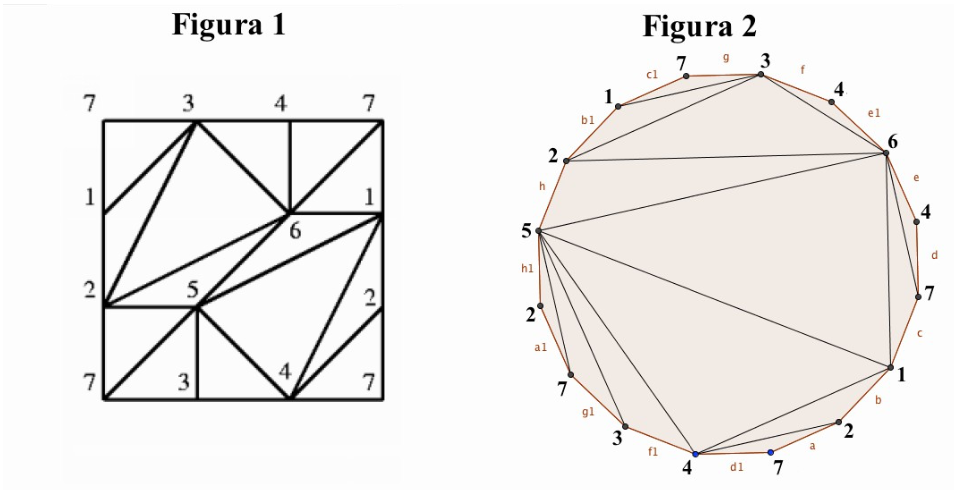
\includegraphics[scale = 0.5]{fotos_topo_2/pinchetriangulacion.png}
\end{equation}
Al fer les identificacions donades per la paraula $B$ obtenim
\begin{equation}
    \notag
    _1a_2b_3c_1d_4e_5e^{-1}_4f_6g_1c^{-1}_3b^{-1}_2h_7h^{-1}_2a^{-1}_1g^{-1}_6f^{-1}_4d^{-1}_1
\end{equation}
és a dir, $v' = 7$ i, per tant, com que la superfície és orientable,
\begin{equation}
    \notag
    g = \frac{1}{2}(1-v'+n) = \frac{1}{2}(1-7+8)=1
\end{equation}
En efecte, veiem que la superfície $S_B = R_{14}$ definida per $B$ és un tor, i així $S_A\simeq S_B$.
\end{ej}




\subsection{Complexos simplicials i complexos cel·lulars}
\begin{defi}
[Complex simplicial abstracte]\label{def:complexsimplicialabstracte}\index{Complex simplicial abstracte} Un \textit{complex simplicial abstracte} és una col·lecció $K$ de subconjunts finits d'un conjunt $V$ tal que si $S\in K$ i $S'\subseteq S$ llavors $S'\in K$, i tal que $\{v\}\in K$ per a tot $v\in V$. Els elements de $V$ s'anomenen \textit{vèrtexs} i els elements de $K$ s'anomenen \textit{cares}. Si $S\in K$, llavors els subconjunts de $S$ es diuen \textit{cares de $S$}.
\end{defi}

Amb aquesta definició hem ``estés'' el concepte de triangle. Per exemple, el triangle estàndard $\Delta$ és, en realitat el 3-símplex estàndard. Més en general, podem definir $\Delta^n$ com la clausura convexa dels punts $e_i:=(0,\ldots,1,\ldots,0)\in \mathbb{R}^{n+1}$ on 1 ocupa el lloc $i$-èsim per a cada $i=1,\ldots,n+1$. Aquest s'anomena $n$-símplex estàndard \index{$n$-símplex estàndard}.

\begin{defi}
[Realització geomètrica d'un complex simplicial]\label{def:realitzaciogeometrica}\index{Realització geomètrica} La \textit{realització geomètrica} d'un complex simplicial abstracte $K$ es denota per $|K|$ i es defineix com l'espai topològic que s'obté prenent una còpia de $\Delta^n$ per a cada cara maximal $\{v_1,\ldots,v_{n+1}\}$ de $K$ i unint aquests símplexs per les seves cares comunes, després de fixar una bijecció entre cada cara maximal de $K$ i els vèrtexs del símplex corresponent. L'espai resultant s'anomena \textit{políedre} o \textit{complex simplicial}\index{Políedre}\index{Complex simplicial}.
\end{defi}

Mirem ara quins són els complexos cel·lulars. Si $X$ és un espai topològic i $f:S^{n-1}\rightarrow X$ és una aplicació contínua, on $n\geq 1$, denotem per $X\cup_f D^n$ l'espai obtingut prenent la unió disjunta de $X$ i una bola tancada $D^n$ i identificant cada punt $z\in\partial D^n$ amb $f(z)$. Direm que aquest espai s'ha obtingut adjuntant una \textit{$n$-cel·la}\label{def:ncella}\index{$n$-cel·la}. De manera anàloga podem adjuntar simultàniament una col·lecció (finita o infinita) de $n$-cel·les a $X$ mitjançant un conjunt d'aplicacions contínues $f_\lambda:S^{n-1}\rightarrow X$, on $\lambda\in \Lambda$, per a qualsevol conjunt $\Lambda$.

\begin{defi}
[Complex cel·lular]\label{def:complexcellular}\index{Complex cel·lular} Un \textit{complex cel·lular} és un espai topològic $X$ juntament amb una descomposició $X = \bigcup_{n=0}^\infty X^{(n)}$ (com a espai topològic), on $S^{(0)}$ és un espai discret (un conjunt de punts amb la topologia discreta) i cada subespai $X^{(n)}$ amb $n\geq 1$ s'obté adjuntant una col·lecció de $n$-cel·les a $X^{(n-1)}$. L'espai $X^{(n)}$ s'anomena \textit{esquelet de dimensió $n$}\label{def:esquelet}\index{Esquelet} de $X$. 
\end{defi}

Si $X = X^{(n)}$ per a algun $n$, llavors direm que $X$ és un complex cel·lular de dimensió $n$. Qualsevol complex simplicial $|K|$ és un complex cel·lular on les $n$-cel·les es corresponen amb les cares $\{v_1,\ldots,v_{n+1}\}$ de $K$.


\subsection{Teorema de classificació de superfícies triangulables}

En (\ref{ter:totasuperficiecompactaestriangulable}) hem vist que tota superfície compacta és triangulable. Això, en particular, ens dona una nova manera de classificar superfícies: ens dóna la possibilitat de classificar totes les superfícies. 

\begin{ter}[Teorema de classificació de superfícies]
\label{ter:teoremadeclassificaciodesuperficies2.0}\index{Teorema de classificació de superfícies} Tota superfície compacta i connexa $S$ és homeomorfa a $S^2$ o a $g\mathbb{T}^2$ si és orientable, i a $g\mathbb{R}P^2$ si no és orientable. 
\end{ter}
\begin{proof}
Sigui $M$ una superfície topològica compacta i connexa. Escollim una triangulació finita de $M$. Aleshores els triangles de la triangulació es poden representar al pla de manera que quedi un polígon amb les arestes de la seva vora identificades per parells. Observem que si alguna aresta de la vora no s'identifiqués amb cap altra, llavors $M$ seria una superfície amb vora i, si tres o més arestes s'identifiquessin entre elles, llavors els punts de l'aresta resultant no tindrien cap entorn homeomorf a $\mathbb{R}^2$.

Tallant i enganxant, aquest polígon es pot convertir en un altre polígon corresponent a la forma normal de $g\mathbb{T}^2$ o bé $g\mathbb{R}P^2$ o bé $\mathbb{S}^2$ mitjançant els passos\footnote{Aquests passos crec que es diuen transformacions de Tietze.} següents:
\begin{enumerate}
    \item Eliminar els parells $aa^{-1}$ consecutius, si n'hi ha. Si el polígon només té dues arestes, llavors és una esfera $aa^{-1}$ o un pla projectiu $aa$ i ja hem acabat. 
    \item Fer que el polígon acabi tenint tots els vèrtexs identificats en un de sol.
    \item Fer consecutius tots els parells $aa$ si n'hi ha.
    \item Agrupar els parells $aa^{-1}$ i $bb^{-1}$, si n'hi ha, passant-los a la forma $cdc^{-1}d^{-1}$.
    \item Utilitzar al final, si és necessari, el fet que $k\mathbb{T}^2\#\ell\mathbb{R}P^2\simeq (2k+\ell)\mathbb{R}P^2$.
\end{enumerate}
\end{proof}


\subsection{Característica d'Euler}

Sigui $\mathcal{T}$ una triangulació d'una superfície $S$ (amb o sense vora). Si la triangulació $\mathcal{T}$ és finita, es denota
\begin{itemize}
    \item $v$ el cardinal dels vèrtexs de $\mathcal{T}$,
    \item $a$ el cardinal de les arestes de $\mathcal{T}$,
    \item $c$ el cardinal dels triangles (les cares) de $\mathcal{T}$.
\end{itemize}

\begin{defi}
[Característica d'Euler]\label{def:caracteristicaeuler}\index{Característica d'Euler} Es defineix la \textit{característica d'Euler} de $\mathcal{T}$ per
\begin{equation}
    \notag
    \chi(\mathcal{T}):=v-a+c
\end{equation}
\end{defi}

Notem que si $\mathcal{T}$ és una triangulació d'una superfície $S$ compacta (sense vora), com cada cara té tres costats i cada costat ho és de les dues cares, tenim $3c = 2a$. Per tant, $c$ és parell i
\begin{equation}
    \notag
    \chi(\mathcal{T})=v-\frac{3c}{2}+c=v-\frac{c}{2}.
\end{equation}

\begin{ej}
\label{ej:caracteristicaeuler} Veiem algun exemple
\begin{enumerate}
    \item Considerem el disc tancat $\mathbb{D}^2 = \{(x,y)\;:\;x^2+y^2\leq 1\}$ i sigui $\mathcal{T}$ la triangulació de $\mathbb{D}^2$ formada pels quatre triangles de $\mathbb{D}^2$ que defineixen els quatre quadrants del pla. Com $\mathcal{T}$ té 5 vèrtexs, 8 arestes i 4 cares, tenim $\chi(\mathcal{T}) = 1$.
    \item El tetraedre regular $T$ dona una triangulació $T$ de l'esfera $\mathbb{S}^2$ que té quatre vèrtexs, 6 arestes i 4 cares. Per tant, $\chi(T)= 2$.
    
    Podem obtenir altres triangulacions de l'esfera amb altres sòlids platònics, i.e. l'icosaedre $I$ té 12 vèrtexs, 30 arestes i 20 cares i, per tant, també $\chi(I)=2$.
\end{enumerate}
\end{ej}

Veurem que qualsevol triangulació de l'esfera té $\chi(\mathcal{T})=2$ i, més generalment, es té el següent resultat.

\begin{prop}
\label{prop:caracteristicaeulerrang} Sigui $S$ una superfície compacta i connexa. Si $\mathcal{T}$ és una triangulació de $S$, aleshores
\begin{equation}
    \notag
    \chi(\mathcal{T}) = 2-\mathrm{rang}\pi(S)
\end{equation}
\end{prop}

Se segueix d'aquest teorema que la característica d'Euler d'una triangulació de $S$ és un invariant de $S$. Per tant, totes les triangulacions de $S$ tenen la mateixa característica d'Euler. Així doncs, podem ara definir la característica d'Euler d'una superfície \index{Característica d'Euler d'una superfície} com la característica d'Euler d'una de les seves triangulacions, i que la triangulació escollida influeix, és a dir, que la característica d'Euler de $S$ és independent de quina triangulació de $S$ es prengui. A més, es té que superfícies homeomorfes tindran la mateixa característica d'Euler.

\begin{proof}
Recordem que si $N$ és el nombre de triangles de $\mathcal{T}$, en el teorema (\ref{prop:triangulacio1}) hem provat que existeix un polígon $P_N$ regular de $N+2$ costats, amb una triangulació $\mathcal{T}_N$ per diagonals internes, i una aplicació $\varphi_N:P_N\rightarrow S$ que indueix un homeomorfisme $P_N/\sim_A\simeq S$ i tal que la triangulació $\mathcal{T}$ de $S$ és la imatge de $\mathcal{T}_N$ per $\varphi_N$. Com la triangulació $\mathcal{T}_N$ té com a vèrtexs els $N+2$ vèrtex de la vora de $P_N$, al identificar els costats de la vora de $P_N$ segons la paraula $A$ per obtenir $S$, els vèrtexs de la triangulació $\mathcal{T}$ de $S$ són els $v'$ punts en els que s'identifiquen els vèrtexs del polígon $P_N$, és a dir, els vèrtexs del graf $G_N$. Per tant, la característica d'Euler de $\mathcal{T}$ és
\begin{equation}
    \notag
    \chi(\mathcal{T}) = v'-\frac{3N}{2}+N=v'-\frac{N}{2},
\end{equation}
i com que en (\ref{prop:triangulaciosuperficies}) hem provat que 
\begin{equation}
    \notag
    \mathcal{rg}\pi(S)=1-v'+\frac{N+2}{2} = 2-v' + \frac{N}{2},
\end{equation}
es conclou que 
\begin{equation}
    \notag
    \chi(\mathcal{T})=2-\mathrm{rg}\pi(S)
\end{equation}
\end{proof}



\begin{coro}
\label{coro:caracteristicaeulerorientabilitat} Sigui $S$ una superfície compacta, connexa i de gènere $g$. Aleshores, si $S$ és orientable,
\begin{equation}
    \notag
    \chi(S) = 2-2g
\end{equation}
i si $S$ és no orientable, aleshores 
\begin{equation}
    \notag
    \chi(S) = 2-g
\end{equation}
\end{coro}
\begin{proof}
En efecte, se segueix immediatament de la relació entre el rang del grup fonamental i el gènere que hem provat a (\ref{prop:triangulacio1}),
\begin{itemize}
    \item si $S$ és orientable, $\chi(S) = 2-\mathcal{rg}\pi(S) = 2-2g$, i
    \item si $S$ és no orientable, $\chi(S) = 2-\mathrm{rg}\pi(S) = 2-g$.
\end{itemize}
\end{proof}

\begin{ej}
\label{ej:caracteristicaeuleresfera} Com que l'esfera $\mathbb{S}^2$ és simplement connexa, $\mathrm{rg}\pi(\mathbb{S}^2)=0$, i així tota triangulació de l'esfera té $\chi(\mathcal{T})=2$.

Veiem com d'aquí se segueix el resultat provat originalment per Euler. 

Si $P$ és un políedre convex, amb $V$ vèrtexs, $A$ arestes i $C$ cares, afegint un vèrtex en l'interior de cada cara, podem obtenir una triangulació $\mathcal{T}$ de $P$ prenent els triangles que defineixen aquests nous vèrtexs i les arestes de $P$. Aquesta triangulació $\mathcal{T}$ tindrà $v = V+C$, $a = 3A$ i $c = 2A$, i per tant,
\begin{equation}
    \notag
    \chi(\mathcal{T}) = v-a+c = (V+C)-3A+2A = V-A+C
\end{equation}
Donat que $P$ és homeomorf a l'esfera $\mathbb{S}^2$, $\chi(\mathcal{T})=2$ i resulta, en definitiva, $V+C = 2+A$, que és la relació provada per Euler en 1758:
\begin{quote}
    \guillemotleft In omni solido hedris planis incluso numerus angulorum solidorum una cum numero hedrarum binario superat numerum acierum.\guillemotright
\end{quote}
(En tot sòlid limitat per cares planes el nombre d'angles sòlids juntament amb el nombre de cares supera en dos al nombre d'arestes.
\end{ej}






















\end{document}